\documentclass[]{thesis-ekf}
\usepackage[T1]{fontenc}
\PassOptionsToPackage{defaults=hu-min}{magyar.ldf}
\usepackage{fancyvrb,listingsutf8,xcolor,caption,graphicx}
\usepackage{amsthm,amsmath,amssymb,listings}
\usepackage[magyar]{babel}
\lstset{
	inputencoding=utf8/latin2,
	language=Java,
	basicstyle=\footnotesize,
	numbers=left,
	breaklines,
	postbreak=\hbox{$\color{red}\hookrightarrow\ $},
	xleftmargin=2cm,
	xrightmargin=2cm,
	backgroundcolor=\color{gray!30},
	frame=tlbr,
	framesep=3pt,
	keywordstyle=\bfseries\color{blue},
	commentstyle=\itshape\color{teal}
}
\theoremstyle{definition}
\newtheorem{definicio}{Definíció}[chapter]
\DeclareMathOperator{\tg}{tg}
\setlength{\headheight}{15pt}
\renewcommand{\lstlistingname}{kód}

\begin{document}
\institute{Természettudományi Kar - TTK}
\title{Arduino robotfejlesztés android alkalmazás használatával}
\author{Bozó Tamás Dániel\\Programtervező informatikus}
\supervisor{Balla Tamás\\}
\city{Eger}
\date{2021}
\maketitle
\tableofcontents
\chapter*{Bevezetés}
\begin{flushright}
	\emph{,,There are an endless number of things to discover about robotics. A lot of it is just too fantastic for people to believe.'' -- Daniel H. Wilson}
\end{flushright}

A mai világban egyre több helyen alkalmaznak robotokat. Akár a munkahelyen a termelés felgyorsítására, az egészségügyben az orvosok segítésére, vagy csak az otthonunkban különböző feladatok elvégzésére. Azért választottam ezt a témát diplomamunkám elkészítéséhez, ugyanis az egyetemi tanulmányaim befejezése utáni célom általános iskolai tanárként elhelyezkedni lakóhelyemen és a diákokkal megismertetni a robotika világát.

Szakdolgozatom témája egy olyan robot építése és programozása, mely egy vonallal kirajzolt pályát képes követni, a pályán található esetleges akadályokat érzékelni és kikerülni, de okostelefon segítségével a felhasználó is képes irányítani. A fejlesztés során igyekeztem egy olyan autóhoz hasonló felépítésre törekedni, amit otthon hobbi felhasználók, de akár általános iskolások is képesek megépíteni a megfelelő felügyelet mellett (erről bővebben olvashatnak a későbbiekben), valamint egy olyan programkód írására, amit könnyen meg lehet érteni és esetleg változtatni/bővíteni.

A telefonos applikáció megvalósítására egy olyan kezelőfelületet akartam létrehozni, mely egyaránt biztosítja a lehetőséget a valós idejű irányításra, valamint a robot működésének monitorozására is.
Programnyelvként a C++-t és a Java-t választottam. A Java egy széles körben elterjedt nyelv, melyet könnyen lehet értelmezni, a C++ pedig az Arduino által támogatott nyelv.

Fejlesztői környezetnek az Arduino IDE és Android Studio nevű alkalmazásokat használtam. Ezen alkalmazásokról \az{\pageref{arduino-IDE}.} és \az{\pageref{android-studio}}.~oldalakon részletesebben olvashatnak.

Jelen dokumentumban kitérek a robot megépítéséhez felhasznált hardverekre, a program megírása során használt fejlesztői környezetekre, valamint programozási nyelvekre, az egyes komponensek/funkciók feladataira, a fejlesztés során szerzett személyes tapasztalataimra, végül egy egyszerű összeszerelési/telepítési útmutatót is csatolok. /Kicsit bővebben kifejteni!!/
\chapter{Arduino és Android bemutatása}
\emph{,,Programming today is a race between software engineers striving to build bigger and better idiot-proof programs, and the Universe trying to produce bigger and better idiots. So far, the Universe is winning'' -- Rick Cook, The Wizardry Compiled}
\section{Az Arduino}
Az Arduino egy szabad szoftveres, nyílt forráskódú elektronikai fejlesztőplatform. Széles tömegek számára elérhető, mivel olcsó, könnyen beszerezhető, egyszerűen programozható és csatlakoztatható más eszközökhöz.
\subsection{A platform felépítése}
A fejlesztői platform az úgynevedett "IDE"-ből és egy Arduino Board-ból áll. Az előbbi segítségével programokat írhatunk és tesztelhetünk a számítógépen, utóbbi pedig egy hardver eszköz, amelyre az elkészített programokat feltölthetjük a számítógépen keresztül, majd az eszközöket vezérelhetünk a segítségével. Az Arduinonak két fő eleme van, ezek a szoftver és a hardver. A szoftvert képezi az IDE, a hardvert pedig a különböző Board-ok és a Shield-ek, melyekről több információt találnak \az{\ref{arduino-boards}}~fejezetben.

Az Arduino lap kereskedelmi forgalomban kapható, előre összeszerelt, vagy otthon összeszerelhető alkatrészcsomagként. Mivel nyílt forráskódú a hardver is, bárki készíthet magának saját változatot belőle, vagy az eredetivel kompatibilis klónt.
\subsection{Elérhető alaplapok}\label{arduino-boards}
Az Arduino Board-ok többféle változatban készülnek, amelyek méretben, a mikrovezérlő típusában, a belső memóriában, a be- és kimenetek számában különböznek. Vannak amelyek rendelkeznek beépített Ethernet, Bluetooth, Wi-Fi csatlakozási lehetőséggel. Jelenleg több Board van forgalomban, ezekből néhány:
\begin{itemize}
	\item Arduino/Genuino UNO
	\item Arduino/Genuino 101
	\item Arduino/Genuino Micro
\end{itemize}
\subsection{Memória és Háttértár}
Egy Arduino három memóriatípussal rendelkezik, melyek különböző feladatokat látnak el.

\textbf{Flashmemória:} A Flashmemória számít az Arduino-k "fő" memóriájának, ez tárolja a letöltött programot, és kikapcsolás után is megőrzi a tartalmát, azaz a programot elegendő csak egyszer letölteni ide, az minden ismételt bekapcsolás esetén "magától" újraindul. Programozás során nem számolhatunk a teljes memóriával, mivel a letöltőprogram (bootloader) és például a különböző kommunikációk is innen "csípnek le" részeket.

\textbf{SRAM:} Az SRAM tárolja a programban definiált belső változókat. Az SRAM - szemben a flash-memóriával - árammentes állapotban nem őrzi meg a tartalmát, ezért minden bekapcsolást követően a program újradefiniálja a változókat és azok az ott meghatározott "alapértelmezett" értékükkel kerülnek az SRAM-ba.

\textbf{EEPROM:} Az EEPROM a board-ok nem felejtő változómemóriája. Ez - hasonlóan a Flash-hez - kikapcsolás során is megőrzi a tartalmát, de - és szintúgy, mint a Flash esetén - "csak" 100.000 írásciklusra van hitelesítve, azaz például a ciklikus adatírásra nem igazán alkalmas. Ráadásul egy kicsit lassabb is a kezelése, mint a "normál" SRAM-é. Ezekből a technikai jellemzőkből adódóan az EEPROM az alábbi funkciókra alkalmazható:
\begin{itemize}
	\item konfiguráció(k) letárolása
	\item indulási alapbeállítások mentése
	\item újraindításoktól független számlálók, értékek, gyűjtött értékek mentése
\end{itemize}
\subsection{Az IDE felépítése és használata}\label{arduino-IDE}
Az Arduino IDE segítségével írt programokat vázlatnak nevezzük. Ezek a vázlatok a szövegszerkesztőben vannak megírva, és az ,,.ino'' kiterjesztéssel kerülnek mentésre. Az IDE teljes felépítése megtekinthető az Arduino hivatalos honlapján\cite{Arduino IDE}.

Az üzenetterület mentés és exportálás közben ad visszajelzést, és megjeleníti a hibákat is. A konzol megjeleníti az Arduino IDE szöveges kimenetét, beleértve a teljes hibaüzeneteket és egyéb információkat. Az ablak jobb alsó sarkában megjelenik a beállított alaplap és soros port.

Az eszköztárban található gombokkal ellenőrizhetjük és feltölthetjük a kódot, új vázlatot hozhatunk létre, valamint megnyithatjuk a soros monitort is.

További parancsok találhatók az öt menüben: \textbf{Fájl, Szerkesztés, Vázlat, Eszközök, Súgó}. A menük kontextusra érzékenyek, ami azt jelenti, hogy csak a jelenleg elvégzett munka szempontjából releváns elemek állnak rendelkezésre.
\subsection{A C++ nyelv}
A C++ egy általános célú, magas szintű programozási nyelv. Támogatja a procedurális, az objektumorientált és a generikus programozást, valamint az adatabsztrakciót. Napjainkban szinte minden operációs rendszer alá létezik C++ fordító.

A nyelv a C programozási nyelv hatékonyságának megőrzése mellett törekszik a könnyebben megírható, karbantartható és újrahasznosítható kód írására, ez azonban sok kompromisszummal jár, erre utal, hogy általánosan elterjedt a mid-level minősítése is, bár szigorú értelemben véve egyértelműen magas szintű.

Bjarne Stroustrup kezdte el a C++ programozási nyelv fejlesztését a C programozási nyelv kiterjesztéseként, más nyelvekből véve át megoldásokat (Simula67, Algol68), ötleteket (ADA).

A nyelv első, nem kísérleti körülmények közt való használatára 1983-ban került sor, 1987-ben pedig nyilvánvalóvá vált, hogy a C++ szabványosítása elkerülhetetlen. Ez a folyamat 1991 júniusában kezdődött el, amikor az ISO szabványosítási kezdeményezés részévé vált.

A C++ programozási nyelv szabványát 1998-ban hagyták jóvá ISO/IEC 14882:1998 néven, az aktuális, 2017-es változat kódjelzése ISO/IEC 14882:2017.
\section{Az Android}
Az Android egy Linux kernelt használó mobil operációs rendszer, elsősorban érintőképernyős mobil eszközökre (okostelefon, táblagép) tervezve. Fejlesztését az ’Android, Inc.’ kezdte el, melyet a Google 2005-ben felvásárolt, majd az Open Handset Alliance folytatta.

A fejlesztők Java vagy Kotlin nyelven írhatnak rá menedzselt kódot, az eszközt a Google által fejlesztett Java programkönyvtárakon keresztül vezérelve.
\subsection{Az operációs rendszer története}
Az Android 1.0 platform 2008. október 21-én került kiadásra Apache licenc alatt, mely nem nyerte el igazán az átlagfelhasználók tetszését, ennek oka a használhatóság nehézsége, illetve a kinézete volt az oka.
\begin{itemize}
	\item 2010-ben a Google bemutatta a Nexus referenciakészülék-termékcsaládját, amit külsős cégek gyártanak. A Google összeállt a HTC-vel, és bemutatták a Nexus One mobiltelefont, amin már az Android 2.1 volt elérhető. Még ebben az évben bejelentették az utódot, amit már a Samsung gyártott, a Nexus S-t, ami már az újabb 2.3-as Androidot futtatja.
	\item 2011 év végén jött az újabb Galaxy Nexus, szintén a Samsung műhelyéből. Ezen már az Android 4.0 Ice Cream Sandwich futott.
	\item 2012 júniusában megjelent az első Nexus tablet, a Nexus 7, majd ezt követte a Nexus 10. Mindkét tableten az Android 4.1 volt megtalálható.
	\item 2012 novemberében jelent meg a Nexus 4, amit az LG gyártott, Android 4.2-vel.
	\item 2013-ban jött az újabb Nexus 5, szintén LG-gyártmány. Ezen az akkor legújabb, Android 4.4 KitKat futott.
	\item 2014 októberében mutatták be a jelenleg legújabb Nexus-t, a Nexus 6-ot (Motorola) és a Nexus 9-et (HTC), amiken az Android 5.0 Lollipop található
	\item 2015 szeptemberében 2 új modell mutatkozott be: az LG által gyártott Nexus 5X és a Huawei által gyártott Nexus 6P, amelyek Android 6.0 Marshmallow-al érkeztek. Ezek után már nem mutattak be újabb Nexus telefonokat, helyüket a Pixel telefonok vették át.
	\item 2016 októberében jelentette be a Google a Pixel és Pixel XL telefonokat, amelyeket a HTC gyártott.
	\item 2017-ben szintén októberben mutatta be a Google a Pixel 2-t, amit újra a HTC gyártott és a Pixel 2 XL-t, amelyet az LG készített.
	\item 2018-ban az eddigiek alapján újra októberben mutatta be a Google a Pixel 3-at és a Pixel 3 XL-t.
\end{itemize}
\newpage

\subsection{Az Android Studio felépítése és használata}\label{android-studio}
Az Android Studio egy integrált fejlesztőkörnyezet (IDE) az Android platformra való fejlesztéshez. 2013. május 16-án jelentette be a Google I/O konferencián Google termékmenedzsere Katherine Chou. Az Android Studio szabadon elérhető Apache License 2.0 alatt.

Az Android Studio első korai szakaszának elérhetősége a 0.1-gyel kezdődött 2013. májusában, majd belépett a béta szakaszba a 2014. júniusában kiadott 0.8 verzióval. Az stabil verziók a 2014. decemberében az 1.0-s verziótól számíthatók.

A JetBrains IntelliJ IDEAján alapuló szoftvert, az Android Studiot kifejezetten androidos fejlesztésre tervezték. Letölthető Windowsra, Mac OS Xre és Linuxra is egyaránt, és teljes egészében helyettesíti az Eclipse Android Development Tools (ADT)-ját. A Google elsődleges IDE-jének választott a natív Android alkalmazás fejlesztésre.

Az új funkciók folyamatosan jelennek meg az Android Studio új kiadásaiban. Minden verzió lehetőséget ad arra, hogy a fejlesztett programot egy virtuális okostelefon segítségével használjuk a számítógépen vagy a csatlakoztatott telefonra telepítsük.
\subsection{A Java nyelv}
A Java általános célú, objektumorientált programozási nyelv, amelyet a Sun Microsystems fejlesztett a ’90-es évek elejétől kezdve egészen 2009-ig, amikor a céget felvásárolta az Oracle. 2011-ben a Java 1.7-es verzióját az új tulajdonos gondozásában adták ki.

A Java alkalmazásokat jellemzően bájtkód formátumra alakítják, de közvetlenül natív (gépi) kód is készíthető Java forráskódból. A bájtkód futtatása a Java virtuális géppel történik, ami vagy interpretálja a bájtkódot, vagy natív gépi kódot készít belőle, és azt futtatja az adott operációs rendszeren. Létezik közvetlenül Java bájtkódot futtató hardver is, az úgynevezett Java processzor.

A Java nyelv a szintaxisát főleg a C és a C++ nyelvektől örökölte, viszont sokkal egyszerűbb objektummodellel rendelkezik, mint a C++. A JavaScript szintaxisa és neve hasonló ugyan a Java-hoz, de a két nyelv nem áll olyan szoros rokonságban, mint azt ezekből a hasonlóságokból gondolhatnánk.

Bár a nyelv neve kezdetben Oak\footnote{James Gosling, a nyelv atyja nevezte így az irodája előtt növő tölgyfáról} volt, később kiderült, hogy ilyen elnevezésű nyelv már létezik, ezért végül Java néven vált ismertté. A Java szó a Oracle védjegye. Ennélfogva engedélye nélkül nem használható mások által kifejlesztett termékek megjelölésére; még például Java-szerű... stb. összetételben sem, mert ez a védjegyjogosult jogaiba ütközik.
\chapter{Követelményspecifikáció}\label{kövspec}
Ebben a fejezetben arról fogok beszámolni, hogy a projekt kigondolásakor, milyen célt tűztem ki magamnak, valamint ennek megvalósítására milyen komponenseket használtam.
\section{Vágyálomrendszer leírása}\label{követelmény}
A projekt megalkotásakor a célom egy olyan robot kifejlesztése volt, amit különböző életkorú diákok, illetve hobbi felhasználók is tudnak használni.

A projekttel szeretném elérhetővé tenni az általános iskolások számára a robotika világának megismerését, de lehetőséget akartam biztosítani azon középiskolás diákoknak is, akik a robotikán túl kihívásra vágynak. Nekik az Android applikáció egy új képesség elsajátítására ad lehetőséget.

Azon személyeknek, akik hobbiból szeretnének egy ilyen robotot megépíteni egy kellemes kikapcsolódás élményét próbáltam biztosítani, ahol maguk építhetik fel a robotot lépésről-lépésre.
\section{Jelenlegi helyzet leírása}\label{jelenlegi_helyzet}
\chapter{Funkcionális specifikáció}
A fejezetben a projekt felhasználási lehetőségeit mutatom be funkcionalitást tekintve, valamint \az{\ref{kövspec}.~fejezetben} \az{\pageref{követelmény}.~oldalon} megfogalmazottaknak feleltetem meg a termékemet.
\section{Arudino}
A robot és az Arduinohoz tartozó program komplexitása könnyen csökkenthető vagy növelhető, ezért többféle felhasználást biztosít.
\begin{itemize}
	\item \textbf{Általános iskola:} A projekt iskolások részére (7-8. osztály) biztosít betekintést a robotika világában. Amennyiben szeretnénk a robotot meg tudjuk építeni úgy, hogy vonalat kövessen, egyenesen mozogjon, de amint akadályt érzékel, egy másik irányba forduljon, vonalat kövessen, akadály kikerülésével. Ezekhez a kód, és a robot felépítését is könnyedén lehet változtatni.
	\item \textbf{Középiskola:} Azon diákoknak javasolt, akik már dolgoztak Arduino-val, nekik az Android fejlesztésbe biztosít alapot. Kezdő Android szinten a projekt módosítható úgy, hogy csak a telefon küldjön adatot a robotnak, aminek hatására az elvégzi a feladatot, későbbiekben az oda-vissza kommunikáció (logolás) is bemutatható.
	\item \textbf{Hobbi felhasználó:} A mellékelt felhasználói útmutató (7.fejezet) alapján a robot összeszerelése, illetve a programok telepítése lépésről-lépésre követhető, ezért nincs szükség előzetes ismeretre, a projekt csupán szórakozási/időtöltési funkciót lát el.
\end{itemize}
\section{Android}
Az applikáció a roboton található komponensektől függően maximum két felhasználási lehetőséget biztosít.
\begin{itemize}
	\item \textbf{Automata követés:} A robot egy meghatározott pályát követ végig, amiről adatokat küld a telefonra (milyen irányba változott a pálya, akadályészlelés történt, ki lett kerülve az akadály, megállt a robot, elindult a robot), továbbá a felhasználó meg tudja állítani és újra el tudja indítani a robotot.
	\item \textbf{Bluetooth vezérlés:} A felhasználó a képernyőn lévő gombok segítségével tudja irányítani a robot mozgását.
\end{itemize}
\chapter{Belső állapotok és felületterv}
\emph{,,Any fool can write code that a computer can understand. Good programmers write code that humans can understand.'' -- Martin Fowler}
\section{A robot belső állapotai}
A robot működése során többször is változik a belső állapota, a változást a telefonos applikációból kapott adat, valamint a roboton található szenzorok idézik elő.
\subsection{Kezdőállapot}\label{kezdokepernyo_allapot}
\begin{figure}[h]
	\centering
	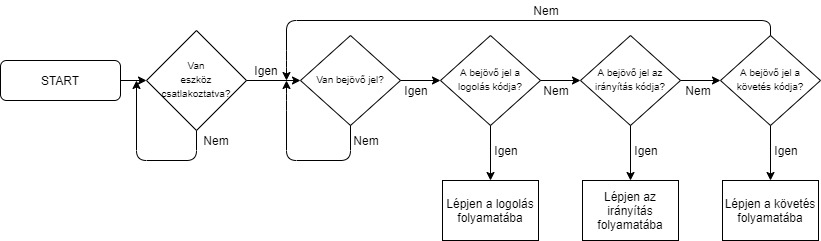
\includegraphics[width=\columnwidth]{images/grafok/fomenu_graf}
	\caption{Kezdőállapot}
	\label{start_allapot}
\end{figure}
A robot indulásakor a kezdőállapotból minden alkalommal a telefonról kapott jel fogja kimozdítani. Amint van csatlakoztatott eszköz a robot elkezdi várni az utasítást. A telefonról érkező utasítás 3 számkód lehet. Minden számkód egy-egy folyamatért felel, mely lehet:
\begin{itemize}
	\item Irányítás folyamata = 111-es kód
	\item Pályakövetés folyamata = 222-es kód
	\item Naplózás folyamata = 333-as kód
\end{itemize}
\subsection{Az irányítás folyamata}\label{controlkepernyo_allapo}
Abban az esetben, ha az applikáció főmenüjében az ’irányítás’ lehetőséget választjuk a robot elkezd várni a bejövő utasításra. Amennyiben ez az utasítás megegyezik a folyamatot megszakító kóddal a robot visszatér a kezdőállapotába.

Ha a kapott utasításból származó kód az 'F', 'L', 'R', 'B', 'S' betűk valamelyike a robot az ehhez tartozó mozgást végzi el.
\begin{itemize}
	\item F = Előrehaladás
	\item L = Balkanyar
	\item R = Jobb kanyar
	\item B = Tolatás
	\item S = Állj
\end{itemize}

A telefon a kódot mindaddig küldi ki a robotnak, amíg az adott gomb lenyomva van. Amint a gombot felengedjük a telefon elküldi a robot megállítására szolgáló 'S' kódot.
\begin{figure}[h]
	\centering
	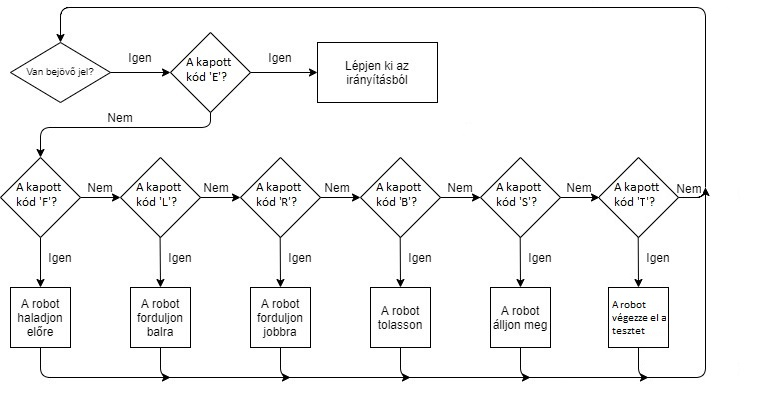
\includegraphics[width=\columnwidth]{images/grafok/iranyitas_graf}
	\caption{Bluetooth irányítás}
	\label{iranyitas_graf}
\end{figure}
\subsection{Automata követés folyamata}\label{followkepernyo_allapot}
Amennyiben a kezdőképernyőn a ’követés’ gombot nyomja meg a felhasználó a roboton található szenzorok végzik el a belső állapotok változtatását.
Ekkor a robot a váz elején található Infravörös szenzorok által érzékelt vonal követését hajtja végre és ebből az állapotából két esetben lép ki:
\begin{itemize}
	\item Valamelyik IR szenzor jelzést ad a vonal kanyarodásáról
	\item Az 'autó' elején található UH szenzor akadályt érzékel
\end{itemize}
\begin{figure}[h]
	\centering
	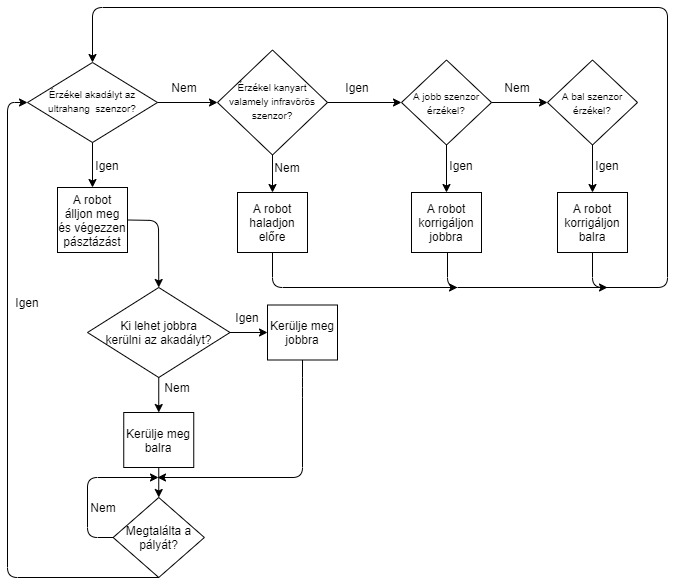
\includegraphics[width=\columnwidth]{images/grafok/kovetes_graf}
	\caption{A követés folyamata}
	\label{kovetes_graf}
\end{figure}

Mindaddig, míg a robot nem érzékel akadályt vagy kanyart a motorok egyforma sebességgel forognak előre. Amennyiben kanyarról ad jelzést valamely IR szenzor a robot korrigálást hajt végre a megfelelő motorok paramétereinek megváltoztatásával (nyomaték, irány). Amint a korrigálás megtörtént és a jelzést leadó szenzor visszaáll eredeti értékére, a robot visszatér a követő állapotba.

Amennyiben akadály érzékelése történik minden motor leállításra kerül, majd a robot elvégez egy pásztázást a váz elején található szervó motor és UH szenzor segítségével. A pásztázás befejezését követően az akadály megkerülése történik jobb vagy bal irányba, majd a pálya megtalálását követően a robot ismét követi azt.
\subsection{A naplózási folyamat}\label{naplokepernyo_allapot}
A naplózási folyamat során a robot csak kommunikációs folyamatokat hajt végre a Bluetooth modul segítségével.\begin{figure}[h]
	\centering
	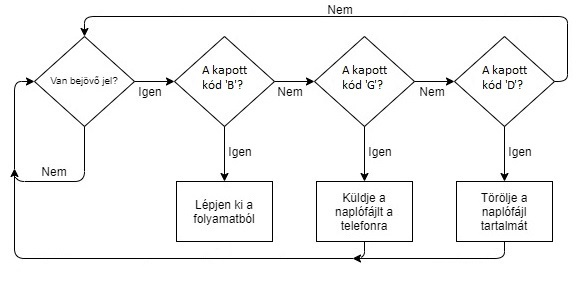
\includegraphics[width=\columnwidth]{images/grafok/log_graf}
	\caption{Naplózási állapotok}
	\label{log_graf}
\end{figure}

Amennyiben a telefonról kapott jel 'B' a robot kilép a folyamatból és \az{\ref{start_allapot}}~állapotba lép.

Ha a bejövő jel 'G' a robot elküldi a telefon részére a Naplófájl tartalmát, ha pedig a jel 'D' törli azt.
\section{Android képernyőtervek}
Az applikációnak négy képernyője van.
\subsection{A kezdőképernyő}
Az alkalmazás elindításakor a felhasználót ez a képernyő üdvözli, ahol öt gomb közül választhatunk, melyek különböző funkciókért felelnek, ezek:
\begin{itemize}
	\item \textbf{Eszközök:} A megnyomása után a képernyőn megjelenik a párosított Bluetooth-eszközök listája, melyből ki tudjuk választani a számunkra megfelelőt.
	\item \textbf{Súgó:} Az applikációba beépített ’Súgó’ képernyő (\ref{help}) válik aktívvá ahol a felhasználó minden funkciót megismerhet.
	\item \textbf{Követés:} Átirányítja a felhasználót az ’Automata követés’ képernyőjére (\ref{auto-follow}).
	\item \textbf{Irányítás:} A felhasználó a ’Bluetooth irányítás’ képernyőre kerül (\ref{bluetooth-control}), ahol a robotot tudjuk vezérelni.
	\item \textbf{Log:} A naplófájl megtekintésére és mentésére szolgáló képernyőre kerül a felhasználó. (\ref{log_screen})
\end{itemize}
\begin{figure}[h]
	\centering
	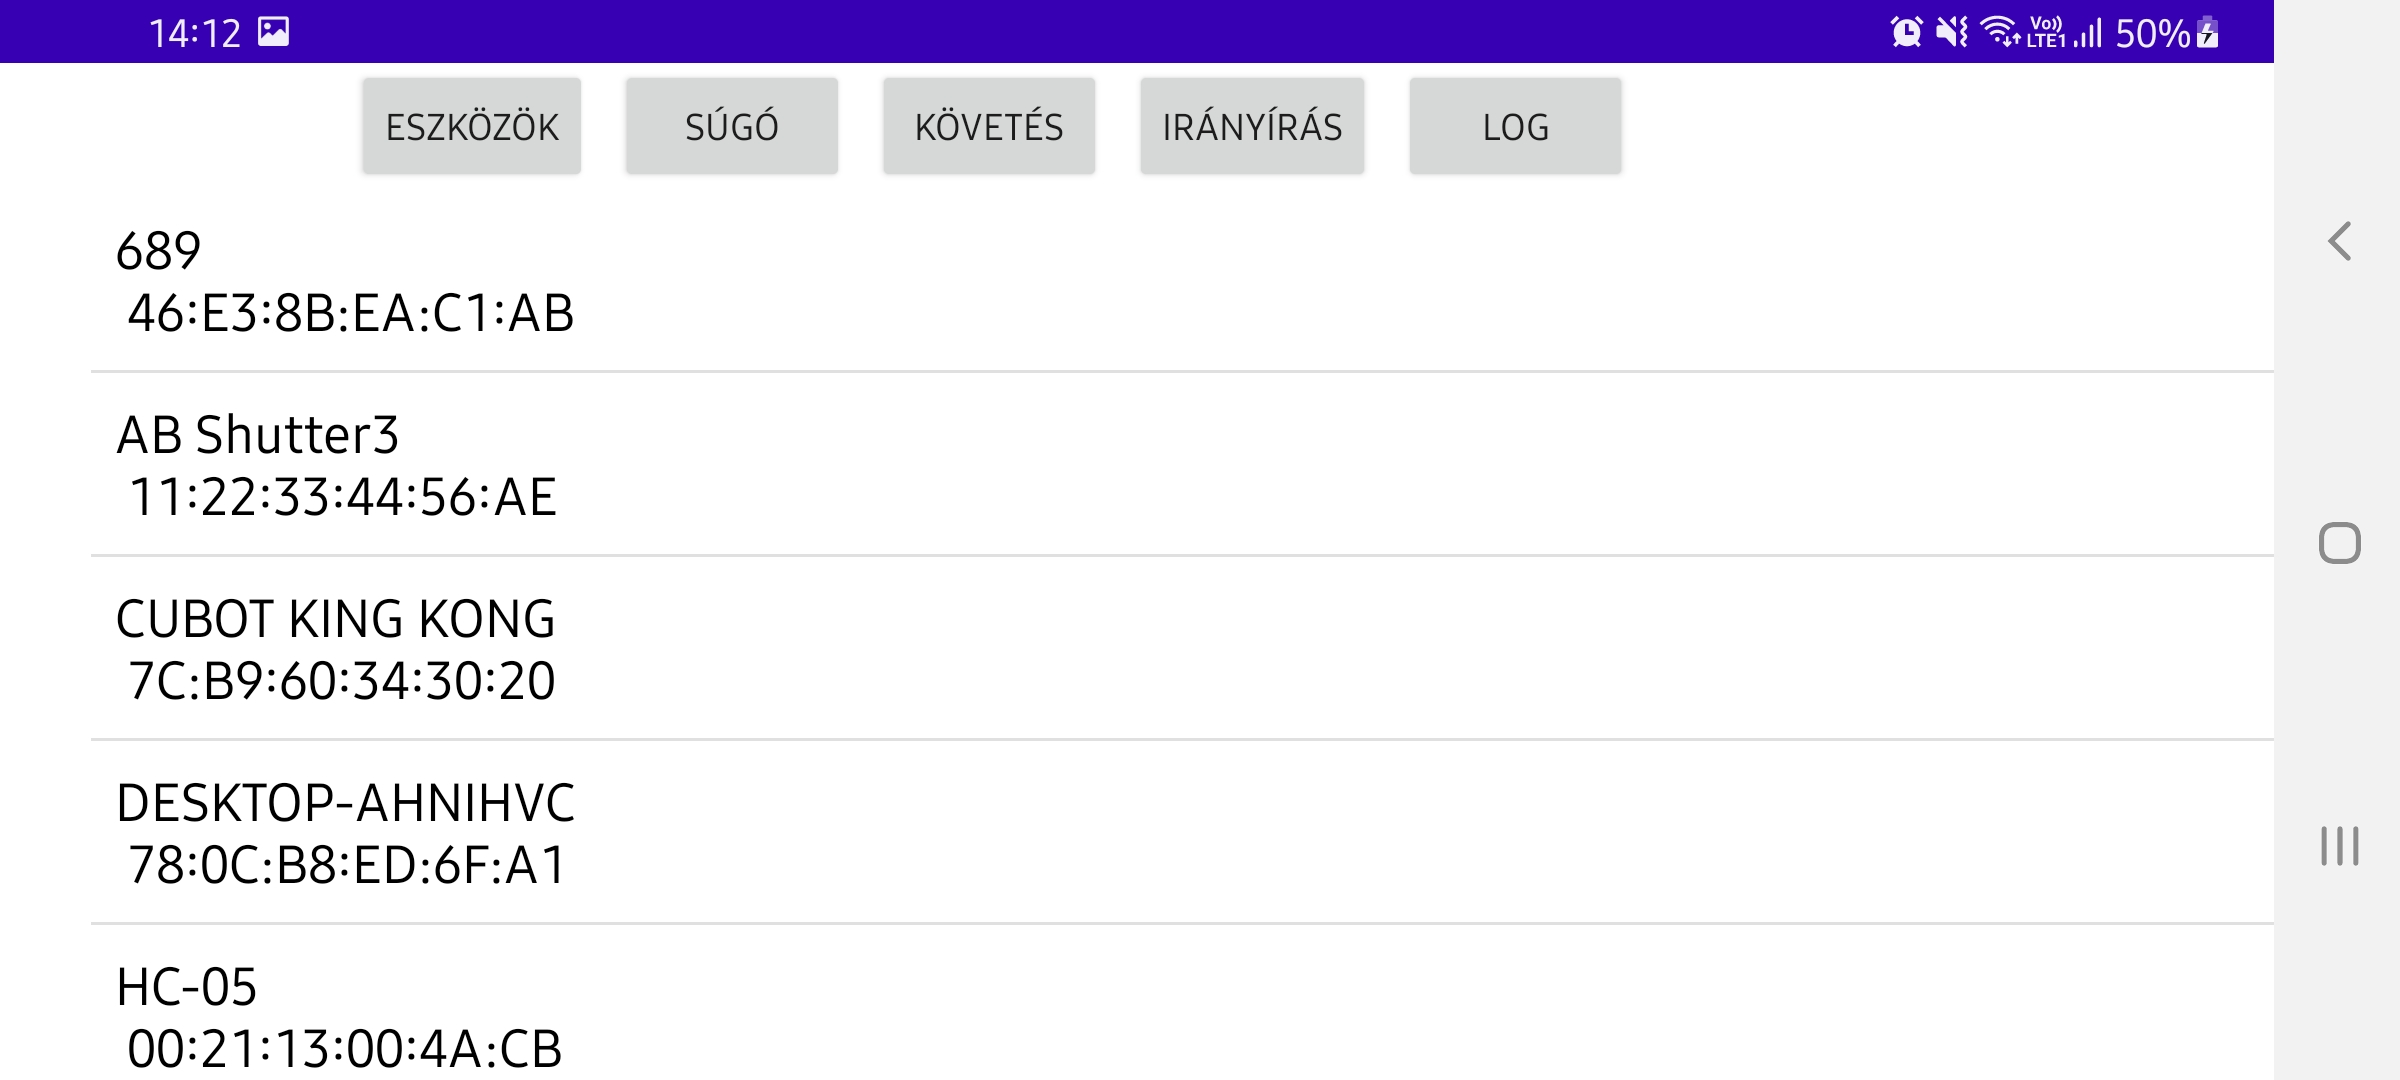
\includegraphics[width=\columnwidth]{images/app_screen/home_screen}
	\caption{Kezdőképernyő}
	\label{home-screen}
\end{figure}
\subsection{Súgó képernyő}\label{help}
A képernyő tartalmazza a funkciók rövid leírását.
\begin{itemize}
	\item \textbf{Home ikon:} A kezdőlapra navigálja a felhasználót.
	\item \textbf{Szöveg felület:} A kiválasztott gomb által tartalmazott leírást jeleníti meg.
	\item \textbf{Követés/irányítás gombok:} Az applikációban található funkciók leírását jeleníti meg a szöveg felületen.
\end{itemize}
\begin{figure}[h]
	\centering
	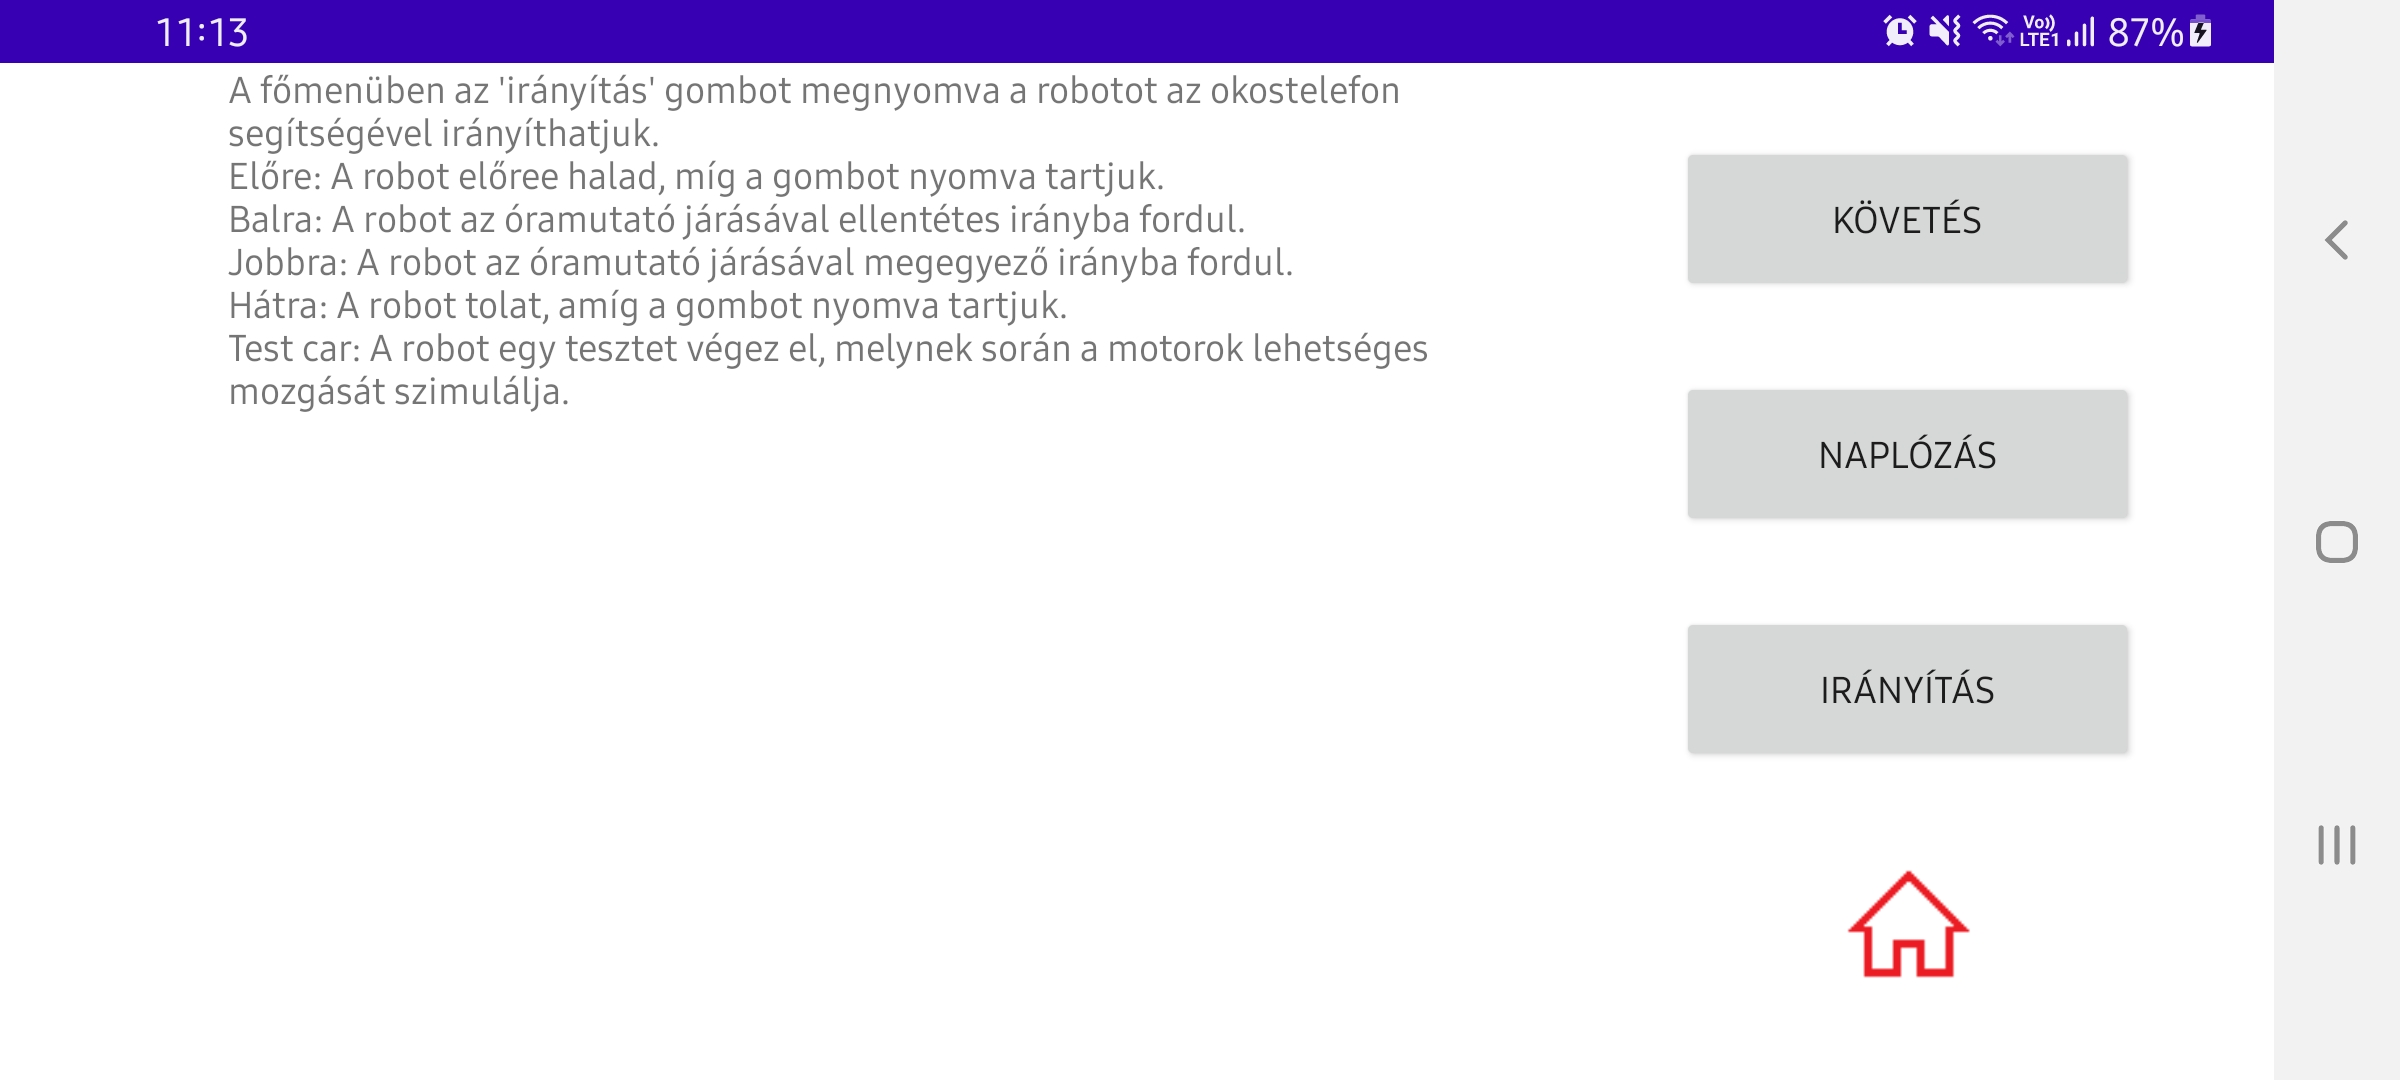
\includegraphics[width=\columnwidth]{images/app_screen/help_screen}
	\caption{Súgó képernyő}
	\label{help-screen}
\end{figure}
\subsection{Az automata követés képernyője}\label{auto-follow}
Amint a felhasználó erre a képernyőre kerül, a robot megkezdi a pálya követését, valamint elérhetővé válnak \az{\ref{follow-screen}~ábrán} látható elemek.
\begin{itemize}
	\item \textbf{’START’ gomb:} Ennek megnyomására a robot elkezdi követni a pályát.
	\item \textbf{'STOP' gomb:} A robot megállítására szolgál.
	\item \textbf{HOME gomb:} A kezdőlapra navigálja a felhasználót, a robot befejezi a pálya követését.
	\item \textbf{SÚGÓ gomb:} Megjelenik a Súgó oldal képernyője.
\end{itemize}
\begin{figure}[h]
\centering
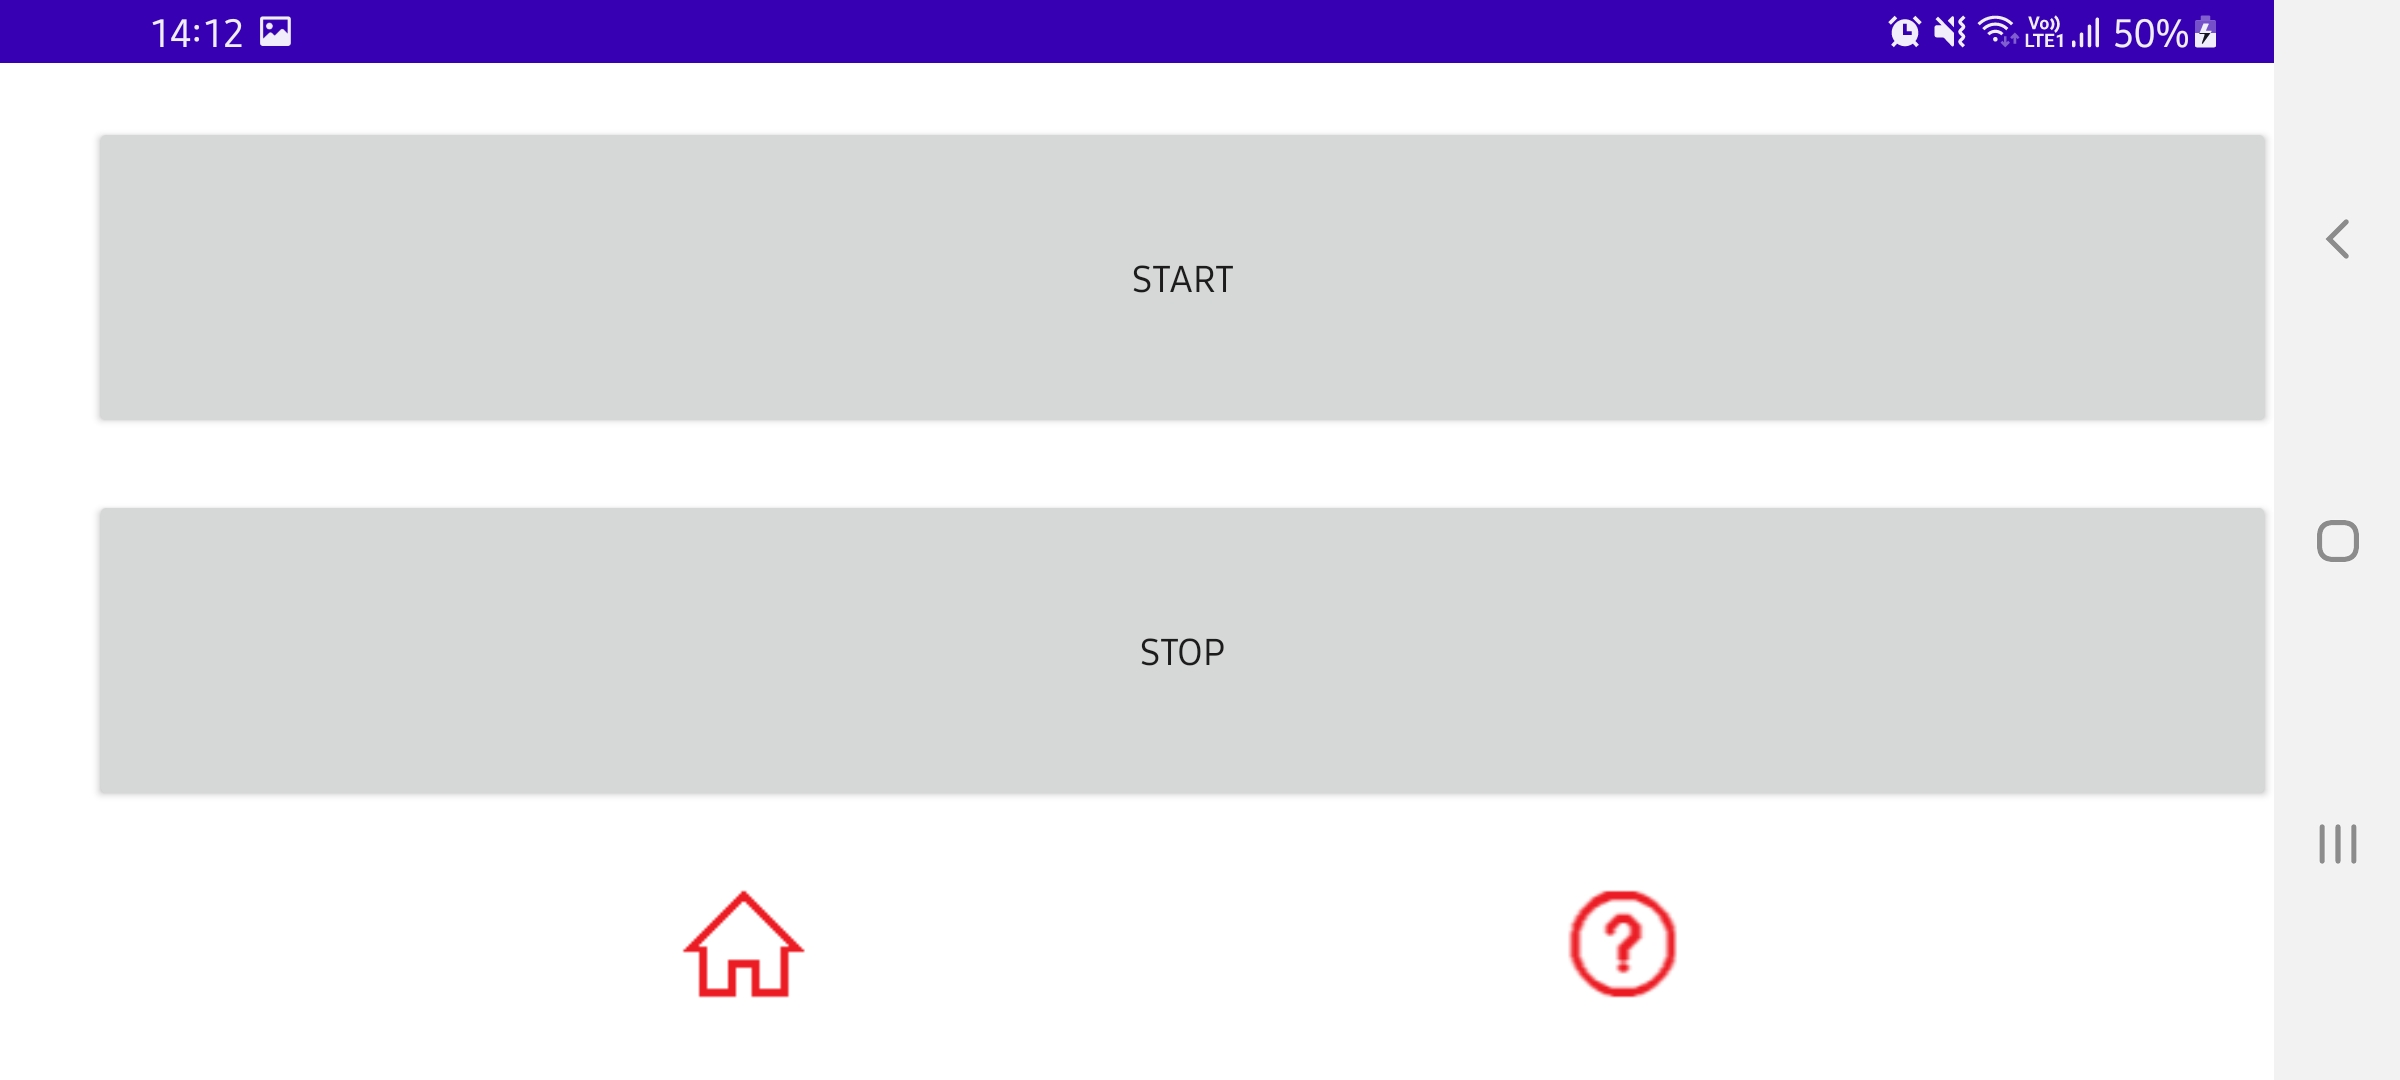
\includegraphics[width=\columnwidth]{images/app_screen/follow_screen}
\caption{Követés képernyő}
\label{follow-screen}
\end{figure}
\subsection{Bluetooth irányítás képernyője}\label{bluetooth-control}
Az ablakon \az{\ref{bluetooth-screen}~ábrán} látható gombok szerepelnek.
\begin{itemize}
	\item \textbf{Előre:} A motorok mindegyike előre halad, megegyező nyomatékkal.
	\item \textbf{Balra: }A roboton található motorok megegyező nyomatékkal, a bal oldaliak hátra, a jobb oldaliak előre forognak, így a robot az óramutató járásával ellentétes irányba fordul.
	\item \textbf{Test car:} A roboton egy előre megírt teszt mozgást futtat le, melynek segítségével a felhasználó ellenőrizni tudja, hogy a motorok működnek-e. A tesztmozgás során a robot minden motorokat érintő mozgást elvégez, melyek:
	\begin{itemize}
		\item Előrehaladás
		\item Tolatás
		\item Jobb kanyar
		\item Bal kanyar
		\item Pásztázás
	\end{itemize}
	\item \textbf{Jobbra:} A roboton található motorok megegyező nyomatékkal, a jobb oldaliak hátra, a bal oldaliak előre forognak, így a robot az óramutató járásával megegyező irányba fordul.
	\item \textbf{Hátra:} A motorok hátra forognak megegyező nyomatékkal.
	\item \textbf{Home:} A kezdőlapra navigálja a felhasználót.
	\item \textbf{Súgó:} A felhasználó a SÚGÓ oldalra kerül.
\end{itemize}
\begin{figure}[h]
	\centering
	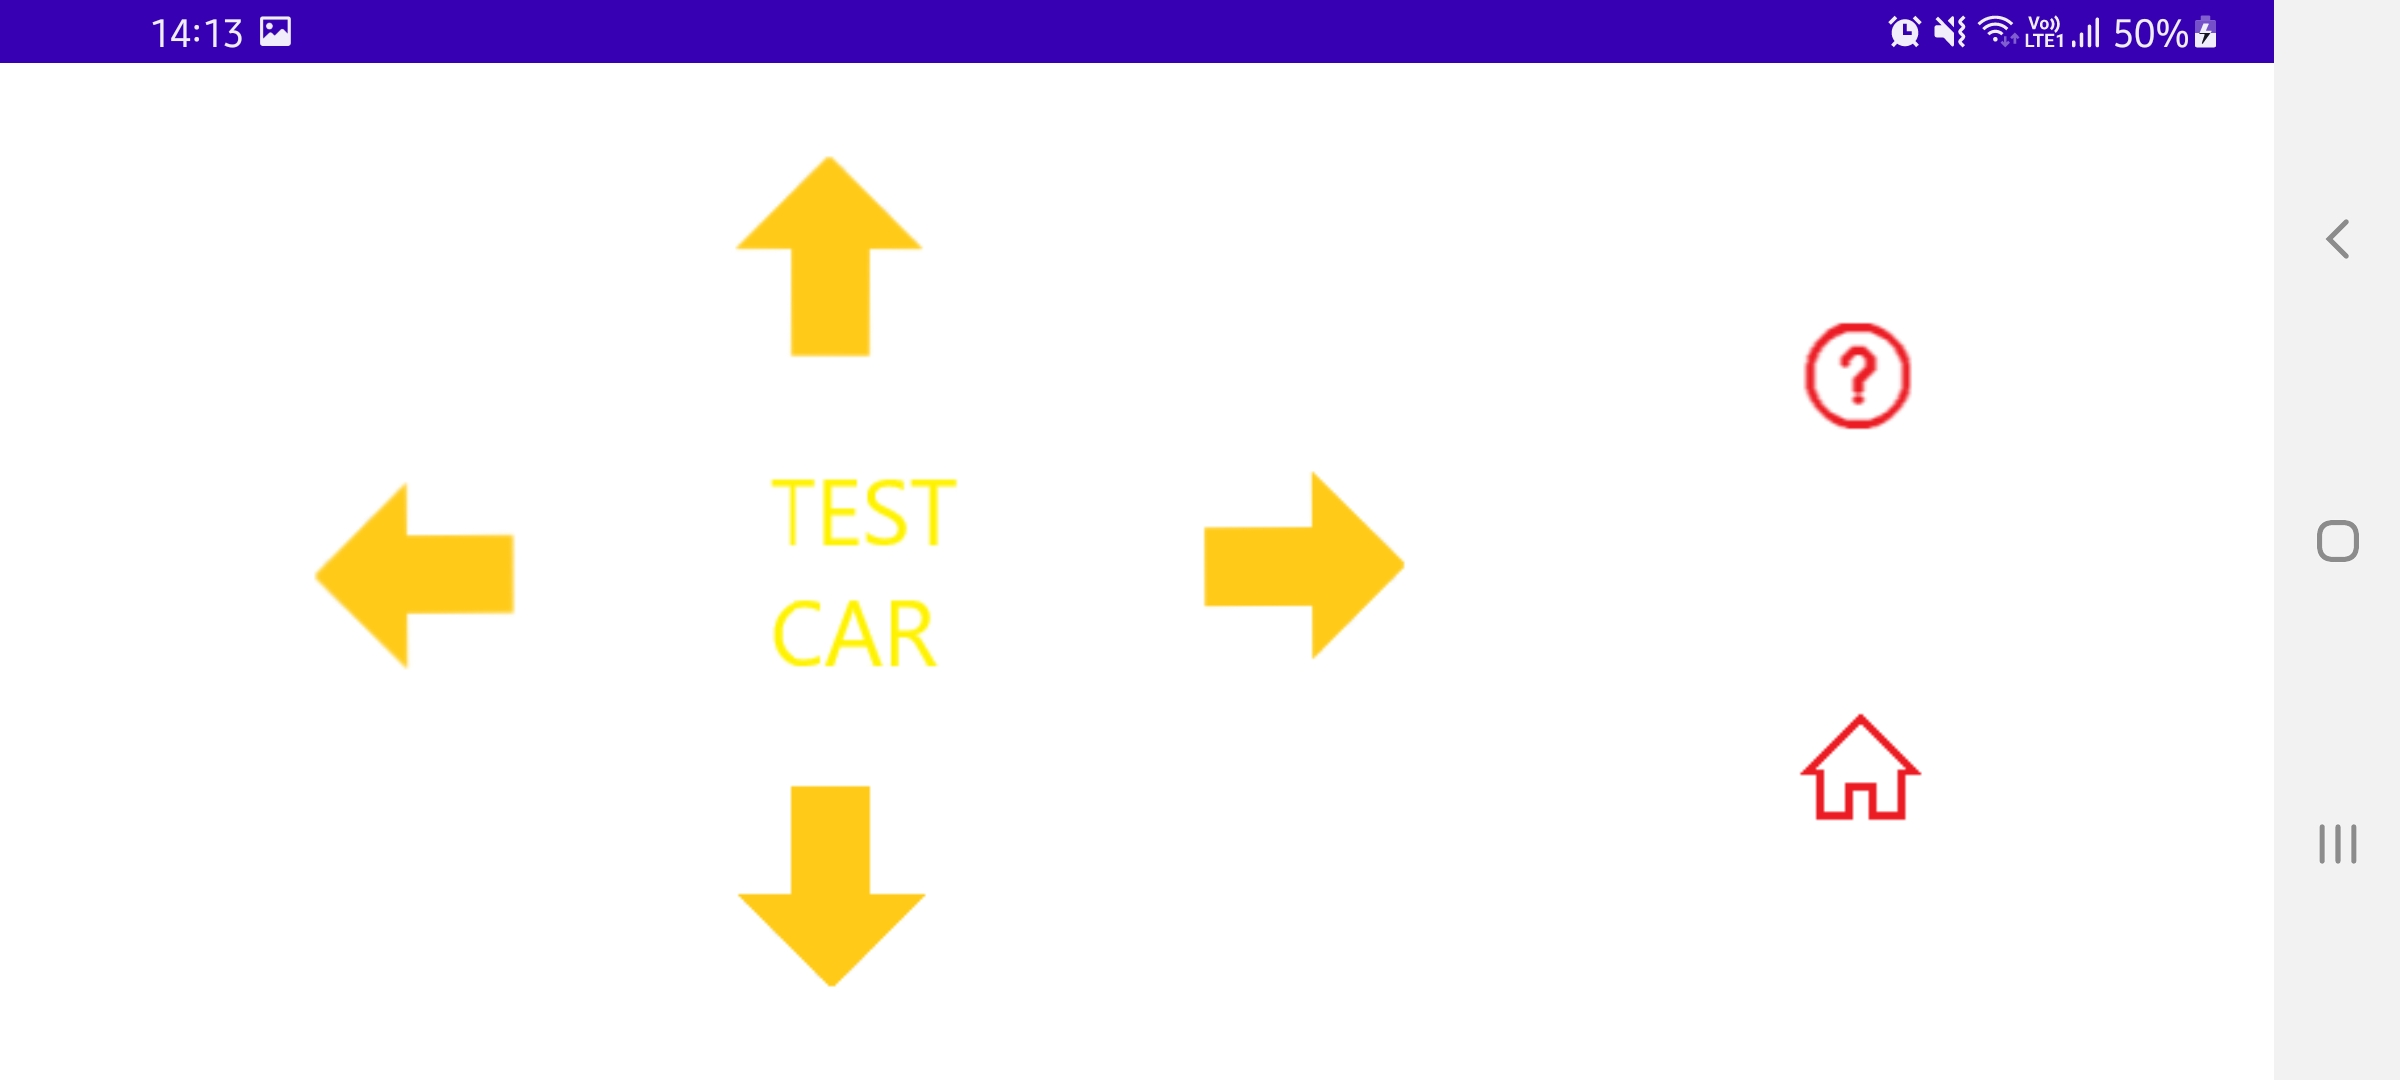
\includegraphics[width=\columnwidth]{images/app_screen/control_screen}
	\caption{Irányítás képernyő}
	\label{bluetooth-screen}
\end{figure}
\subsection{Naplózási képernyő}\label{log}
Ezen a képernyőn tudjuk lekérni a robot által rögzített naplót, valamint ezt tudjuk menteni és törölni is.
\begin{itemize}
	\item \textbf{Log lekérése:} A robottól bekérjük a log fájl jelenlegi tartalmát, majd ezt megjelenítjük a 'Log felület'-en.
	\item \textbf{Log mentés:} A megjelenített napló fájlt a telefonra mentjük a jelenlegi dátumot és időt felhasználva fájlnévként.
	\item \textbf{Log törlés:} A log tartalma törlésre kerül a 'Log felület'-ről, valamint a robot memóriájából is.
\end{itemize}
\begin{figure}[h]
	\centering
	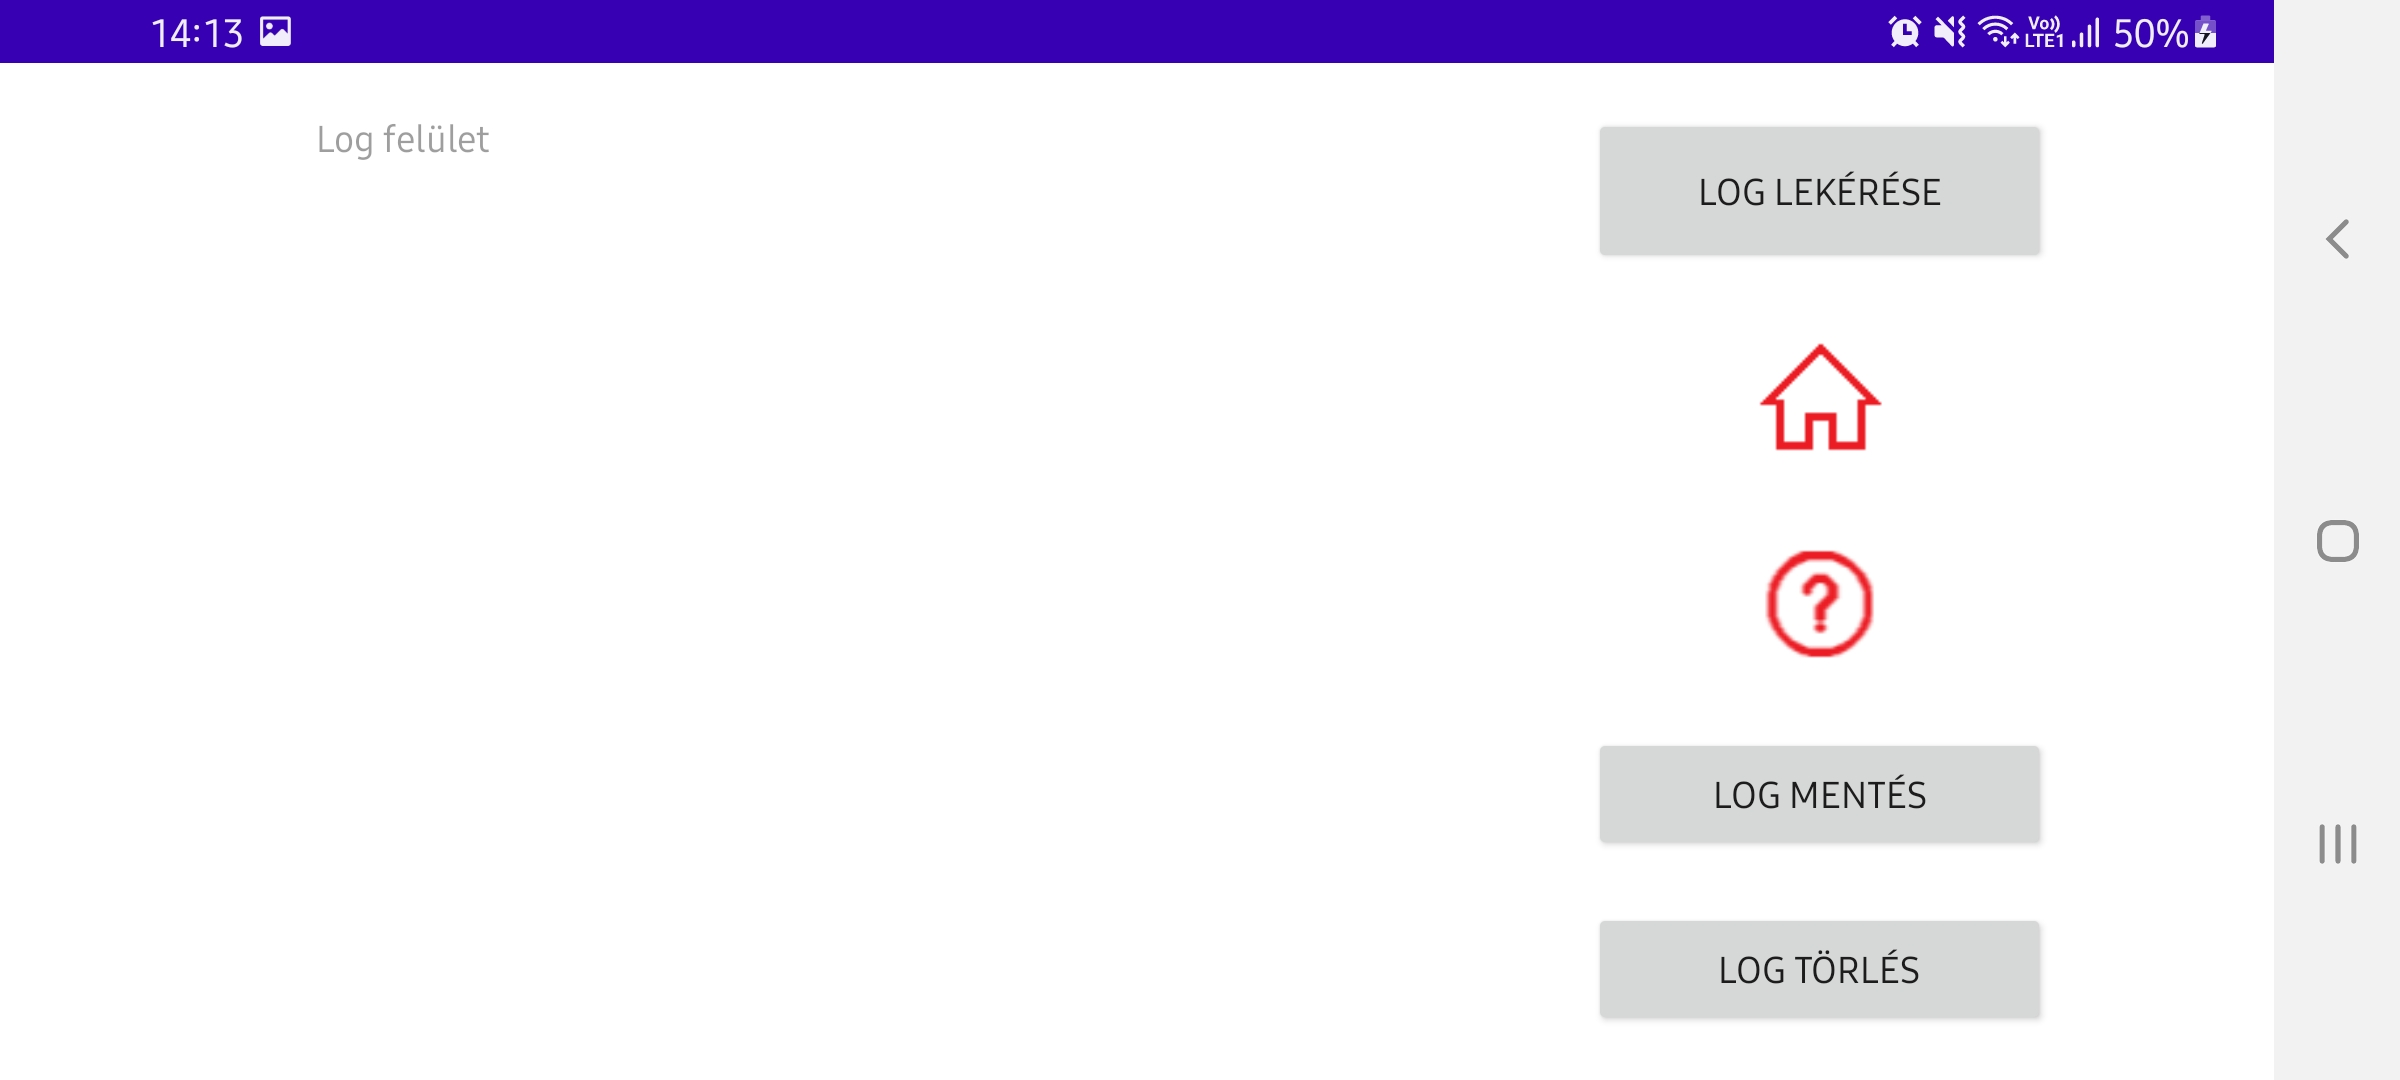
\includegraphics[width=\columnwidth]{images/app_screen/log_screen}
	\caption{Naplózási képernyő}
	\label{log_screen}
\end{figure}

A képernyőn megtalálható \textbf{Home} és \textbf{Súgó} gombok megnyomásakor egy üzenet jelenik meg, mely azt biztosítja, hogy a felhasználó ne felejtse el menteni a log fájlt.

Minden képernyő elérhető horizontális és vertikális elrendezésben, ezzel biztosítva a felhasználó számára a lehetőséget, hogy a neki legkényelmesebb módon tudja tartani készülékét az applikáció használata közben.
\chapter{A robot és az applikáció működése}
\emph{,,In some ways, programming is like painting. You start with a blank canvas and certain basic raw materials. You use a combination of science, art, and craft to determine what to do with them.'' -- Andrew Hunt}

Ebben a fejezetben bemutatom a robot és a telefonos applikáció működését.
\section{A telefon és a robot összekapcsolása}
Mivel a robot a telefonról kapott kód alapján kezdi el valamely folyamatot először szükséges a kettő közötti kapcsolatot biztosítani. A robot kódjában ehhez nem kell mást tenni, csak \az{\ref{arduino_bt_connection}~kódban} látható módon mindaddig, míg a HC-05-ös modulon nincs csatlakozás érzékelve a robotot váratjuk egy while() ciklus segítségével.
\lstinputlisting[caption=Bluetooth csatlakozás\label{arduino_bt_connection}]{codes/arduino/connection.ino}

A telefonos applikációban ennél összetettebb kódra van szükség. Először biztosítani kell azt, hogy az készüléken be legyen kapcsolva a Bluetooth modul, ezt úgy tudtam elérni, hogy egy erre beépített metódust használtam\cite{Bluetooth_active} (\ref{device_choose}~kód 9. sor), és amennyiben ez igaz értéket adott vissza jeleztem a felhasználónak, majd meghívtam a 'BluetoothAdapter.ACTION\_REQUEST\_ENABLE' metódust\cite{Bluetooth_enable}, mellyel a felhasználó engedélyezni tudja a bekapcsolást. 
\lstinputlisting[caption=Eszköz kiválasztása\label{device_choose}]{codes/android/Connectbluetooth.java}

Miután a Bluetooth be van kapcsolva és a felhasználó megnyomta a kezdőoldalon megtalálható gombok valamelyikét az ehhez tartozó megfelelő 'activity' kerül elindításra, valamint ennek paraméterként átadjuk az eszköz adatait is.

A kiválasztott képernyőre való átnavigáláskor rögtön elindul a \ref{device_connect}~kódrészletben megtalálható metódus, mellyel egy előre csatlakoztatott Bluetooth eszközhöz kapcsolódunk. A kapcsolódás folyamata alatt egy állapotjelző látható a képernyőn, majd a csatlakozási folyamat végén a felhasználó  visszajelzést kap a kapcsolat állapotáról.
\lstinputlisting[caption=Bluetooth kapcsolódás\label{device_connect}]{codes/android/BTConnecting.java}
\section{A fő folyamatok eldöntése}
Ahogy a \ref{start_allapot}~ábrán is látható a robot az indulás után három fő állapotba léphet át, melyek az applikációban való képernyőváltással idézhetők elő. Minden alkalommal, mikor a kezdőképernyőt elhagyjuk és a Bluetooth csatlakozás végbe ment az applikáció automatikusan kiküldi az aktív képernyőhöz tartozó aktiváló kódot a robot részére (lásd \ref{kezdokepernyo_allapot}~fejezet), valamint a képernyő elhagyásakor a megszakító kódot is.

Ahhoz, hogy a telefonról képesek legyünk adatok küldésére az 'AndroidManifest.xml' fájljában engedélyeznünk kell a Bluetooth modul használatát melyet a ,,<uses-permission android:name="android.permission.BLUETOOTH" />'' paranccsal tudunk megtenni.
\section{Kód küldése a telefonról}
Az alkalmazásban két módon kell kódot küldeni a robot számára.
\begin{itemize}
	\item Adott gomb lenyomásakor egy alkalommal
	\item Folyamatosan, míg az iránygombok valamelyikét nyomva tartjuk
\end{itemize}

A kód egyszeri kiküldését egyszerűen egy 'onClickListener' használatával el lehet érni, ahol a gomb lenyomásakor \az{mBTSocket} névvel példányosított BluetoothSocket 'getOutputStream().write()' metódusának segítségével elküldjük a kódot.

Az iránykód folyamatos küldéséhez az 'onClickListener' helyett 'onTouchListenert' kell használni. Az utóbbinál a gombtól kapott 'MotionEvent' alapján tudjuk eldönteni, hogy az adott gomb jelenleg le van-e nyomva (ACTION\_DOWN) vagy sem (ACTION\_UP). Ameddig a gomb nyomva van az 'mBTSocket.getOutputStream().write()' metódus segítségével az iránykódot küldjük a robotnak, majd mikor felengedésre kerül a gomb ugyanezen metódussal elküldjük a motorok leállítására szolgáló 'stopAction()' kódját.
\section{Motorok kezelése}
A roboton található 4db villanymotor és 1db szervo motor kezelésére egy motorvezérlő panelt használtam, mely L293D típusú motorvezérlőt tartalmaz. A kódban minden motort külön kell kezelni.
\lstinputlisting[caption=Motorok kezelése\label{motor-shield}]{codes/arduino/motor-shield.ino}

A kódban láthatóan ahhoz, hogy a panelt használni tudjuk meg kell hivatkozni az 'AFMotor' és 'Servo' könyvtárakat.

A könyvtárak hivatkozása után inicializáljuk a 4 motort, melyhez meg kell adnunk, hogy melyik porthoz csatlakozik, illetve azt is, hogy milyen típusú motorról van szó.

Miután a DC motorok példányosítása megtörtént, megtesszük ezt a szervo motorral is. A program 'setup()' részében a 'myservo.attach()' utasítással tudjuk megadni, hogy melyik port felel a szervo motorért. -- Jelen esetben ez a digitális 10-es port lesz.

Amennyiben ezek megtörténtek a szervo motort a 'myservo.write()' utasításban paraméterként megadott értékkel tudjuk forgatni 0-180° között, a DC motort pedig \az{\ref{forward}~kódban} látható módon tudjuk kezelni. -- 'FORWARD' helyett használhatunk 'BACKWARD' parancsot, hogy hátra forgassuk a motort, illetve 'RELEASE' parancsot a motorok leállítására. 

Az \ref{turndetect}~kódban látható 'rightAction()' és 'leftAction()' metódusok meghívásakor nem egy, hanem két értéket kell megadnunk, melyek az előre és a hátra forgó motorok sebességeiért felelnek, míg a 'stopAction()' metódusban nincs szükség érték megadására, ugyanis ez az összes DC motort leállítja, vagyis a sebesség minden esetben 0 lesz.
\lstinputlisting[caption=Előrehaladás\label{forward}]{codes/arduino/forward.ino}
\section{Akadályok érzékelése}
\begin{figure} [!h]
	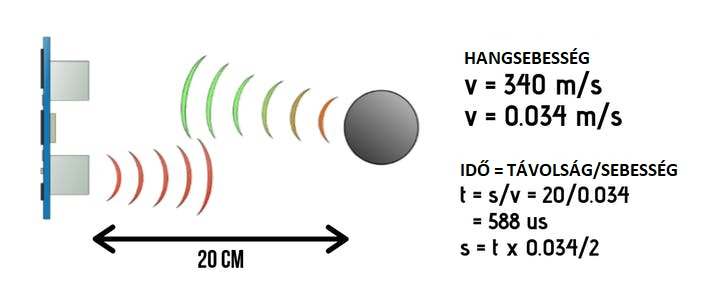
\includegraphics[width=\columnwidth]{images/ultrasonic}
	\caption{HC-SR04}
	\label{ultrahang}
\end{figure}
Ahogy \az{\ref{ultrahang}~ábra} is mutatja a roboton található ultrahang szenzor a jel kiküldése és annak visszaérkezése között eltelt idő alapján határozza meg a távolságot. Mivel tudjuk, hogy a hang levegőben való terjedési sebessége 0.034 cm/µs\footnote{centiméter/mikroszekundum}, a távolságot meg tudjuk határozni úgy, hogy a mért időt megszorozzuk ezzel a sebességgel, majd az így kapott értéket elosztjuk kettővel. -- A kettővel való osztásra azért van szükség, mert a kiküldött jelnek az akadály és a szenzor között oda-vissza meg kell tennie az utat.

A programban ezt \az{\ref{ultrasonic-code}~kódrészletben} látható módon egy metódusba építettem annak érdekében, hogy a kód átlátható legyen.
\lstinputlisting[caption=Akadályérzékelés\label{ultrasonic-code}]{codes/arduino/ultrasonic.ino}
\section{A pályát jelölő vonal követése}
\lstinputlisting[caption=Pálya követése\label{turndetect}]{codes/arduino/linefollow.ino}

Ahhoz, hogy a robot követni tudja a pályát jelölő fekete vonalat kettő HW-201 típusú infravörös szenzort használtam. Abban az esetben, ha a szenzorok valamelyike jelez a vonal kanyarodásáról a robot a megfelelő irányba történő korrigálással reagál, melynek kódja \az{\ref{turndetect}~kódrészleten} látható.

A kódban látható 'forwardAction()', 'backwardAction()', 'leftAction()', 'rightAction()' és 'stopAction()' metódusokban megy végbe a motorok irányítása.
\section{Akadály kikerülése}
A robot programozása közben szükségesnek találtam azt, hogy az autó el tudja dönteni melyik irányba tudja kikerülni az érzékelt akadályt.

Erre \az{\ref{180°-sonar}~kódrészlet} tartalmazza a megoldást. A kódrészletben látható, hogy amint egy akadályt érzékelünk a motorok megállításra kerülnek, majd meghívásra kerül az 'ObstacleAvoidance()' metódus, melyben az alábbi módon történik az akadály kikerülése.
\lstinputlisting[caption=Pásztázás\label{180°-sonar}]{codes/arduino/sonar.ino}
Először meghívjuk a 'backwardAction()' metódust annak érdekében, hogy a kerekek egyike se ütközzön neki az akadálynak.

Ezután megvizsgáljuk a bal és jobb oldalakat és eltároljuk a szenzorral kapott értékeket, amik alapján el lehet dönteni melyik irányba kell kikerülni az akadályt. Az 'if' és 'else' ágakban található metódusok felelnek ezért.

Az akadály kikerülésekor fontos, hogy a robot el tudja dönteni, hogy mikor érte el az akadály szélét. Ennek elérésére egy egyszerű do-while ciklust használtam, melyben a robot addig halad előre, míg az akadály aktuális távolsága maximum 5cm-el haladja meg az eredeti mért távolságot.

Ezek után ismételten meg kellett találni az akadály szélét, hogy széltében is meg tudjuk kerülni azt.

Az akadály kikerülése után a robotnak ismételten meg kell találnia a követendő vonalat. Ezt úgy tudtam elérni, hogy a robot egyenesen halad mindaddig, míg valamely infravörös szenzor jelzést nem ad a vonal érzékeléséről és a robot a jelzést leadó szenzorral ellentétes irányba fordul.
\section{A naplófájl feldolgozása és mentése}
A robot működés közben az adott eseményeket egy 'string' típusú változóban tárolja el a \ref{log_process}~kódrészletben látható módon. Az adat átküldésre a telefonra a 'println()' metódussal történik az applikáció pedig a 'getInputStream()' metódussal fogadja ezt és ezek után már feldolgozhatjuk az adatot, hogy a kívánt módon tudjuk megjeleníteni azt.
\lstinputlisting[caption=Naplófájl feldolgozása\label{log_process}]{codes/android/LogProcess.java}

Miután az adatot fogadtuk, feldolgoztuk és megjelenítettük a felhasználónak lehetősége van menteni is ezt. A mentést a \ref{log_screen}~ábrán látható 'Log mentése' gombbal tudja megtenni a felhasználó. A naplófájl neve az adott dátum lesz másodperc pontossággal, amelynek megvalósítását a \ref{log_save}~kódban láthatnak.

A fájlnév eltárolása után példányosítunk egy új 'FileOutputStream' egyedet, majd ennek paraméterben megadjuk a mentendő fájl nevét és mentési módját.

Ezek után szükség van egy 'OutputStreamWriter' példányra, hogy a létrehozott fájl tartalmát módosítani tudjuk. Ha létrehoztuk a saját egyedünket a beépített 'write()' metódusát használva a fájl tartalmát módosítjuk a LogFelület tartalmával.
\lstinputlisting[caption=Napló mentése\label{log_save}]{codes/android/LogSave.java}

Ahhoz, hogy a fájlt létre lehessen hozni és módosítani tudjuk a tartalmát a megfelelő engedély biztosítása szükséges.

Ehhez engedélyt kell kérni a felhasználótól, hogy az alkalmazás hozzáférhessen a telefon tárhelyéhez. Az engedély megadásához először ellenőriznünk kell, hogy az alkalmazás rendelkezik-e az engedéllyel. Ezt a \ref{storage_permission}~kódrészletben látható beépített metódussal lehet megtenni, majd a kérés után fel is kell dolgozni a felhasználó által hozott döntést, amire az 'onRequestPermissionsResult' metódust kell használni.

Amennyiben a felhasználó nem adja meg az engedélyt a naplófájl mentése nem megy végbe, helyette egy üzenet jelenik meg a képernyőn, mely 
\lstinputlisting[caption=Engedély kérés\label{storage_permission}]{codes/android/StoragePermission.java}
\chapter{Fejlesztés közbeni tapasztalatok}
A fejlesztés közben több hardver és szoftverszintű új tapasztalatot is szereztem. Hardver szinten előfordultak problémák is elsősorban a robotnál az egyes elemek rögzítése kapcsán.
\section{Hardverrel kapcsolatos tapasztalatok}
Nem csak a robot hardvere jelentett néha problémát, hanem a használt telefoné is. A \ref{label}~fejezetben bővebben olvashatnak arról, hogyan befolyásolja a telefon hardvere a projekt teljesének működését.
\subsection{A robot építésekor szerzett tapasztalatok}
A robot fejlesztése közben a legnagyobb problémát a megfelelő alváz megtalálása jelentette.
Amikor eldöntöttem, hogy milyen robotot szeretnék építeni meglátogattam különböző fórumokat, hogy nagyjából megtudjam milyen mennyiségű szenzorra, illetve motorra lesz szükségem.
\begin{figure}[h]
	\centering
	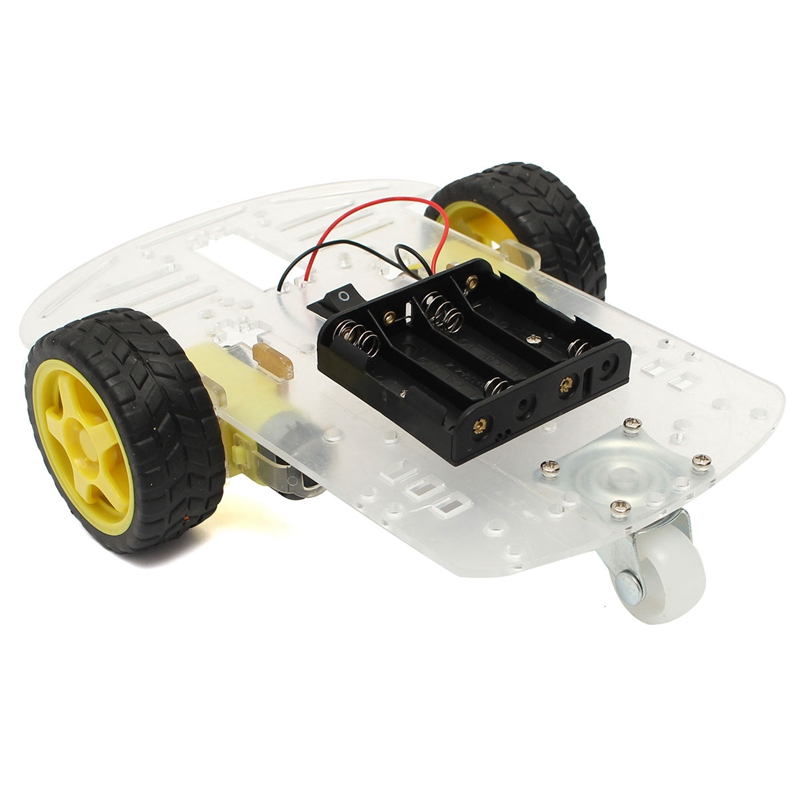
\includegraphics[width=0.4\linewidth]{images/robot_build/2_wheel_car}
	\caption{Két kerekű Arduino alváz}
	\label{2_wheeler}
\end{figure}

Sok már létező projektben a \ref{2_wheeler}~képen látható alvázat használták 'autó' építésére, azonban felmerült bennem a kérdés, hogy hogyan tudom rögzíteni a szükséges infravörös szenzorokat, valamint lesz-e elegendő hely minden szenzornak és az alaplapnak is, ezért úgy döntöttem, hogy ehelyett a megoldás helyett egy saját alvázat használok 4 villanymotorral.

Az alváznak elég nagynak kellett lennie ahhoz, hogy a motorok elférjenek rajta, viszont túl nagy se lehetett, ugyanis egy nagy alváz magában hordozhatja azt a hibalehetőséget, hogy a motorokat nagy nyomatékkal kell használni, hogy a robot mozogni tudjon és ez hamar merítené le az akkumulátort.

Továbbá olyan alváz használatát részesítettem előnyben, mely nem vezeti az elektromosságot, mivel a használt Arduino UNO alaplap alján a forrasztási pontok szabadon vannak felmerült bennem az a kérdés, hogy biztonságos-e egy olyan alváz használata, mely vezető vagy félvezető, vagy esetleg zárlatot fog-e ez okozni.

Miután nem találtam egy fórumon se konkrét választ erre a kérdésemre úgy döntöttem, hogy műanyag alvázat használok.

A robot első verziójának megépítése után azonban rájöttem arra, hogy az alváznak merevnek is kell lennie. Az első tesztek során arra lettem figyelmes, hogy vannak alkalmak amikor a robot minden probléma nélkül képes bevenni egy kanyart, majd a következő alkalommal amikor ehhez a kanyarhoz ér már nem.

Ennek oka az volt, hogy a műanyag alváz rugalmassága és a középen elhelyezkedő akkumulátor súlya miatt a kerekek nem teljes felületükkel érintkeztek a talajjal és ezért a tapadásuk is csökkent.

Mivel nincs birtokomban 3D nyomtató mellyel egy olyan alvázat tudnék nyomtatni, mely merevsége és mérete is megfelelő úgy döntöttem, hogy egy plexi lemezt fogok használni (másik alternatíva lehet a plexi lemeznél olcsóbb SAN\footnote{sztirol-akril-nitril} lemez is). A plexi használatát több okból is jó választásnak tartom.
\begin{itemize}
	\item A merevsége miatt nagy terhelés alatt sem deformálódik, így a kerekek minden esetben teljes felületükkel fognak a talajjal érintkezni
	\item Amennyiben módosítani kell a kinézetét rövid melegítés után lehet hajtani/formázni, miközben nem kell attól tartanunk, hogy eltörik
\end{itemize}

Miután az alvázat kiválasztottam a használt kábelek elvezetésére/védelmére kellett megoldást találnom. Ezt azért tartottam fontosnak, mert ha szabadon vannak a kábelek előfordulhat, hogy a robot olyan helyen halad át, ahol valami ezekbe beleakadhat, így kimozdítva a helyéről, vagy a tüskét, melyhez csatlakozik elhajlíthatja.

Ennek megoldására az alvázra több lyukat is fúrtam, melyek segítségével a kábeleket az alváz alján tudom elvezetni a szenzortól/motortól az alaplapig, továbbá nem használtam hosszabb kábelt, mint amire szükségem volt.
\subsection{A telefon hardverére vonatkozó tapasztalatok}
A fejlesztés során a \pageref{label}~oldalon található specifikációkkal rendelkező telefont használtam, melynél nem tapasztaltam problémát, azonban egy régebbi készüléken az alkalmazás Memoria és energiafogyasztása is jelentősen megnőtt.
\chapter{Továbbfejlesztési lehetőségek}
\emph{,,Always code as if the guy who ends up maintaining your code will be a violent psychopath who knows where you live'' -- John Woods}
\section{Hardverre vonatkozó fejlesztés}
Ahogy \az{\ref{jelenlegi_helyzet}~fejezetben} is olvasható a robot jelenleg nem képes az éles kanyarok precíz bevételére. Ennek megoldását nyújthatja, ha a vonal érzékelésére másfajta szenzort használunk (pl.: Digitális Vonalkövető szenzor), mely pontosabban képes érzékelni a pálya vonalában végbemenő változást.
Lehetséges megoldási módszer a motorok más formában való kezelése az IR szenzorról kapott jelzéskor (nagyobb nyomaték azokra a motorokra melyeknek előre kell mozdulni).

További hardver fejlesztés lehet egy kamera beépítése a robot elejére és ezt felhasználva az irányításért felelős okostelefonon élő képet kaphatunk arról, hogy a robot éppen merre jár. Ennek segítségével a telefonnal való irányításkor nincs szükség arra, hogy a robotot ténylegesen lássuk, hanem a kamera képére hivatkozva ki tudjuk kerülni az akadályokat, valamint egy jobb felhasználói élményt biztosít. Ehhez szükséges egy olyan telefon, amely kellő hardverrel rendelkezik egy ilyen program futtatásához, valamint a külső akkumulátor is gyorsabban fog merülni.
\section{Android szoftverre vonatkozó fejlesztés}
A szoftverben két nagy fejlesztési lehetőségre lettem figyelmes:
\begin{itemize}
	\item Logolás fejlesztése (hardver fejlesztése is szükséges)
	\item Súgó felület bővítése
\end{itemize}
Amennyiben beépítésre kerül a robotra egy Giroszkóp meg lehet mondani, hogy az egyes kanyarok elvégzésekor a robot milyen szögben fordult jobbra/balra, illetve az is, hogy a felületben milyen változás történik (a robot emelkedőn halad felfele, vagy lejtőn lefele).

Ezeket az adatokat felhasználva el lehet készíteni egy statisztikát, valamint automata követéskor a kanyarodások közötti időeltérés és a kanyarok szögének ismeretében a pálya vizualizálása is lehetségessé válhat.

Továbbá amennyiben a felhasználó nincs birtokában a felhasználói útmutatónak (\ref{felhaszn-útmutató}.~fejezet) a robot összeszerelésekor nem tudhatja, hogy az adott szenzort/motort hova kell csatlakoztatnia. Erre megoldást nyújt az említett dokumentum integrálása az applikáció 'Súgó' felületére.
\section{A hardver biztosítására vonatkozó fejlesztés}
A projekt jelenlegi állapotában fedetlenül található meg az összes szenzor, kábel, motor és a mikrokontroller is, ezért fenáll az esélye annak, hogy valamely komponens megsérül, ezzel meggátolva a robot megfelelő működését.

Ennek kijavítása lehetséges egy olyan váz megtervezése és 3D nyomtatása, mely védelmet biztosít a hardver elemeinek, illetve így egy olyan kinézetet lehet adni a robotnak, ami ténylegesen egy autó vázára hasonlít.
\chapter{Felhasználói útmutató}\label{felhaszn-útmutató}
\section{A robothoz tartozó feladatok}
A következő rész tartalmazza a robot megépítéséhez szükséges alkatrészek listáját, ezek bekötési módját, valamint a program telepítésének lépéseit. Fontos megjegyezni, hogy amennyiben a felhasználó hibásan köti be valamely alkatrészt, úgy a robot nem megfelelően fog működni!

\subsection{Szükséges alkatrészek}
A robothoz szükséges elemek.

\begin{center}
	\begin{tabular}{|l|c|}
	\hline
	\multicolumn{1}{|c|}{\textbf{Megnevezés}}&\textbf{Mennyiség}\\
	\hline
	Arduino Uno mikrokontroller&1db\\
	\hline
	Alaplappal kompatibilis L293D-t tartalmazó shield&1db\\
	\hline
	HC-SR04 ultrahang szenzor&1db\\
	\hline
	HW-201 infravörös szenzor&2db\\
	\hline
	SG90 szervo motor&1db\\
	\hline
	Bluetooth modul&1db\\
	\hline
	Villanymotor&4db\\
	\hline
	Kapcsolóval ellátott akkumulátor tartó&1db\\
	\hline
	18650-es akkumulátor&2db\\
	\hline
	Anya-anya jumper kábel&15db\\
	\hline
	1mm átmérőjű sodort rézvezeték ~12-17 cm hosszú&8db\\
	\hline
\end{tabular}
\end{center}
Szükséges továbbá 1db tartóelem az ultrahang szenzor szervó motorra való rögzítéséhez, 1db minimum 15x20cm méretű merev műanyag lap az alváznak, valamint a forrasztáshoz szükséges eszközök.
\subsection{A motorok csatlakoztatása}
Helyezzünk a 4db villanymotor közül egyet magunk elé úgy, hogy a csatlakozási pontok felfele nézzenek, majd ezekhez forraszunk hozzá egy-egy vezetéket. Ha végeztünk ismételjük meg a lépést a többi motorral is. (lehetőség szerint a bal oldali csatlakozóhoz fekete, a jobb oldalihoz piros vezeték kerüljön).
\begin{figure}[h]
	\centering
	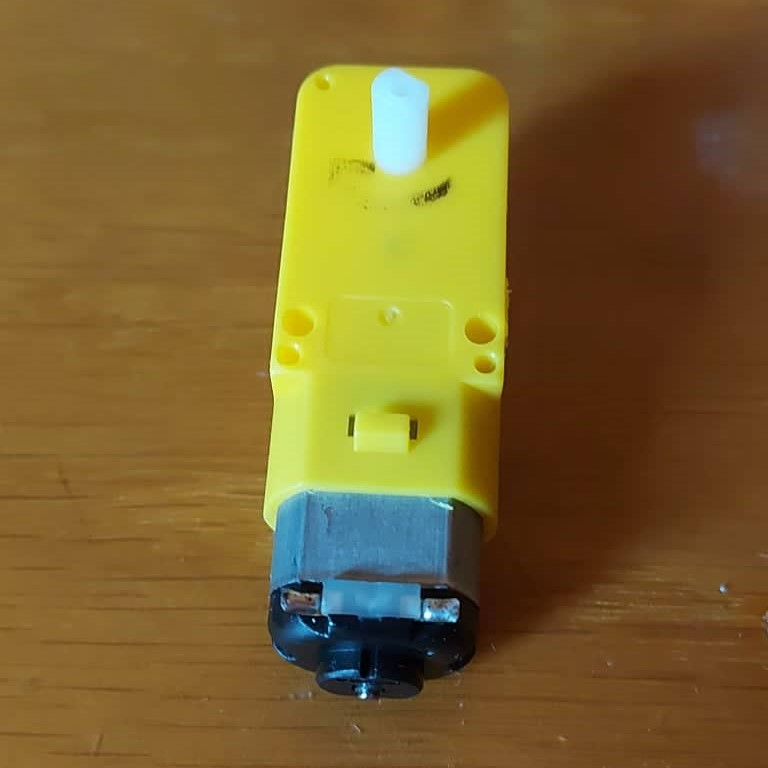
\includegraphics[width=5cm]{images/robot_build/motor-no-cable}
	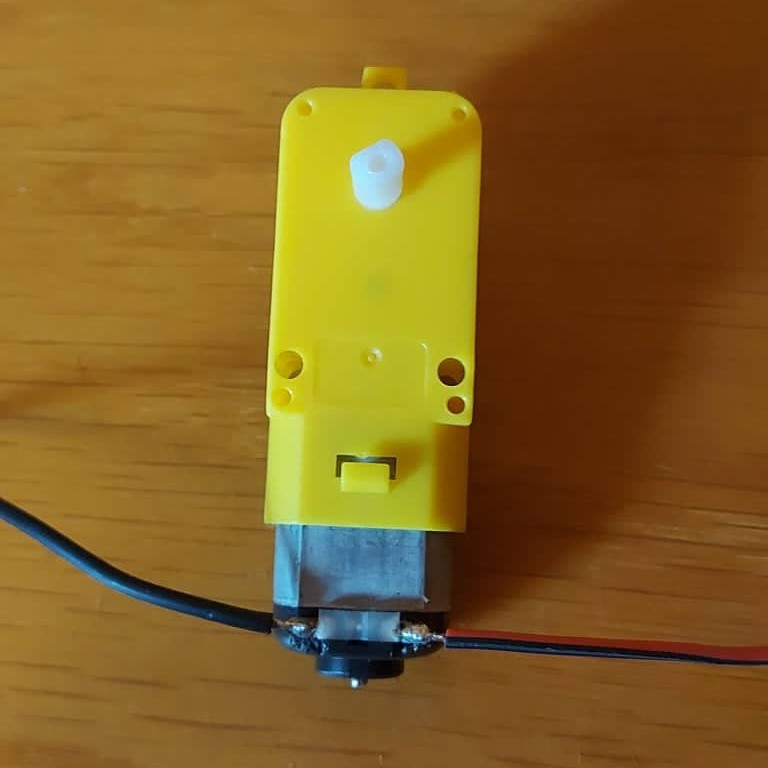
\includegraphics[width=5cm]{images/robot_build/motor-with-cable}
	\caption{A kábelek felhelyezése}
	\label{motor-handling}
\end{figure}

Ezek után a motorokat felhelyezhetjük az alvázra, majd a vezetékeket \az{\ref{shieldre-bekotes}~ábrán} látható módon csatlakoztassuk a motorvezérlő shield-hez.
/Shield-en jelzett M1 – Jobb első, M2 – Bal első, M3 – Bal hátsó, M4 – Jobb hátsó kerékért felelős motor./
\begin{figure}[h]
	\centering
	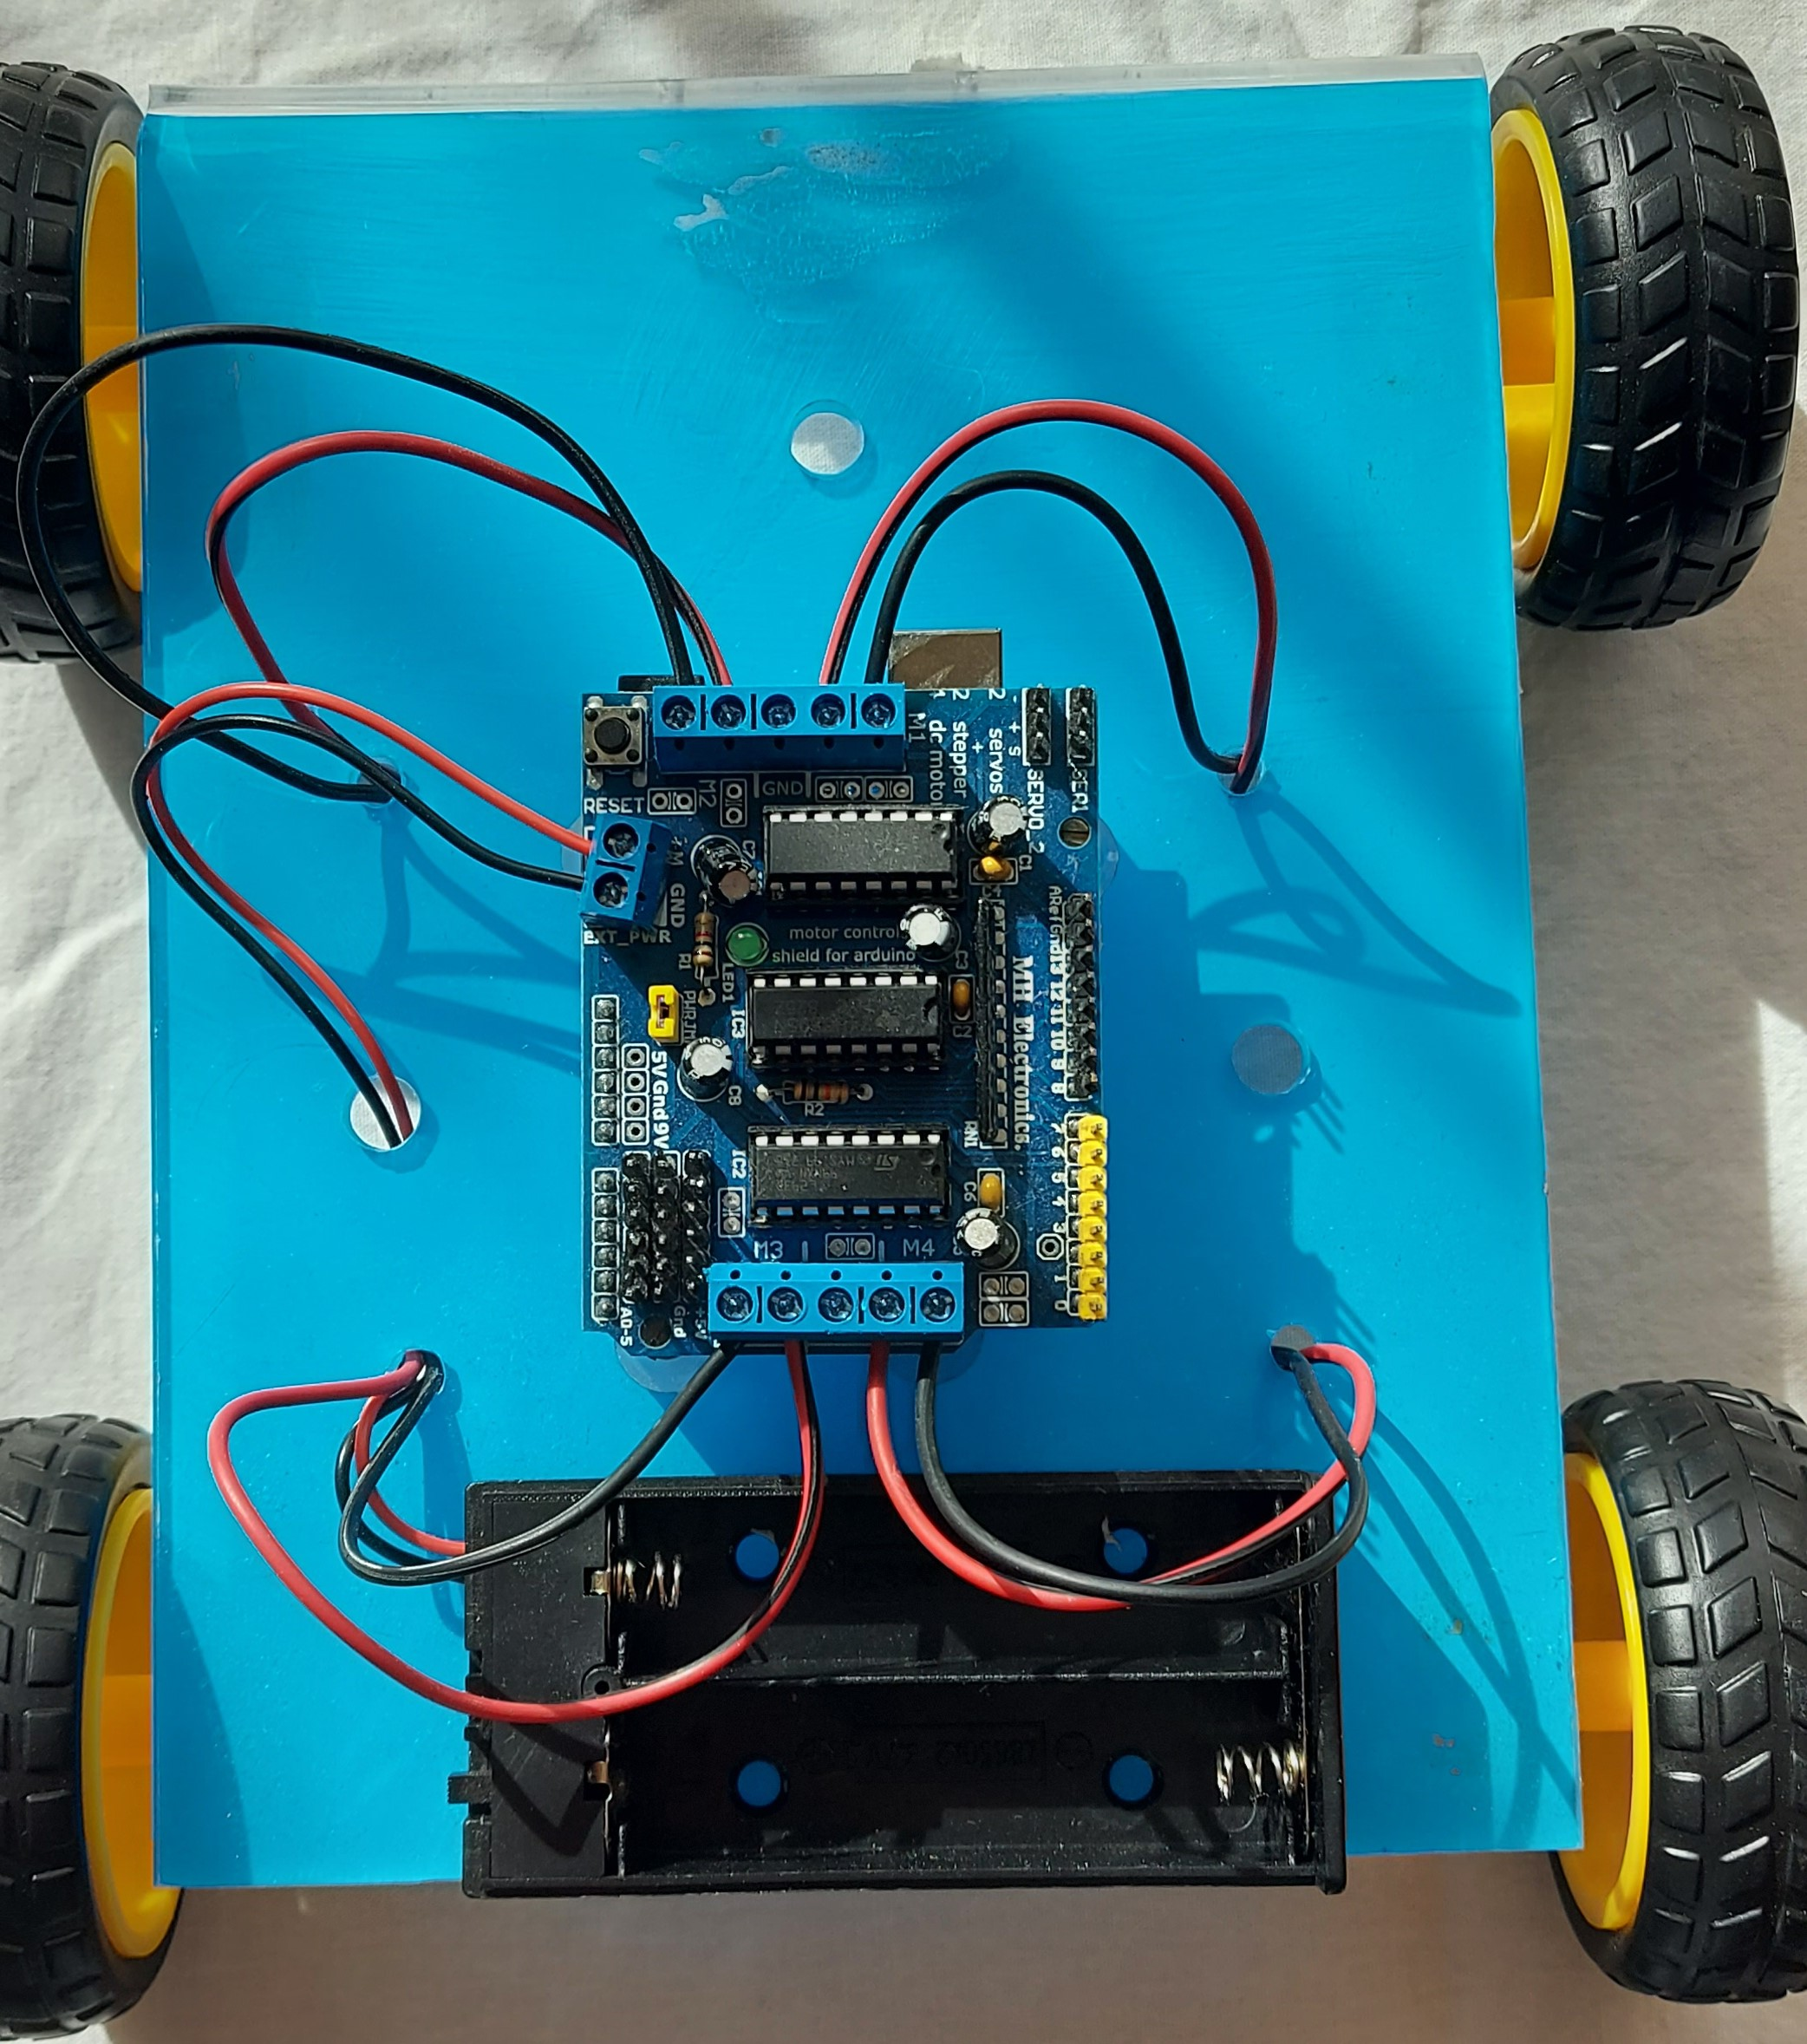
\includegraphics[width=5cm]{images/robot_build/shieldre-bekotes}
	\caption{A shield-re való bekötés}
	\label{shieldre-bekotes}
\end{figure}

\subsection{Szenzorok felhelyezése}
Helyezzük fel az ’autó’ elejére a 2db Infravörös szenzort úgy, hogy a szenzorok között legalább 2-4 cm távolság legyen (a szenzorok közötti távolság méretét a követendő vonal vastagsága határozza meg), majd jumper kábel segítségével csatlakoztassuk ezeket a shield-en található A0 és A1-es, valamint az ehhez tartozó GND és VCC jelölésű portokhoz. (szemből nézve jobb oldali szenzor A0, bal oldali A1).

Ezek után helyezzük fel a szervó motort a szenzorok közé, majd erre a tartóelemet, a hozzá rögzített ultrahang szenzorral. Az ultrahang szenzor ’Trig’ és ’Echo’ jelzéssel ellátott tüskéit csatlakoztassuk a digitális 0 és 1 portokhoz, valamint GND és VCC tüskéit egy-egy GND és VCC porthoz. A szervó motor vezetékét csatlakoztassuk a shield-en található SERVO\_2 jelzésű tüskesorhoz.

A korábbi lépések elvégzése után helyezzük fel a Bluetooth modult, majd csatlakoztassuk a TX -- Transmitter és RX -- Receiver tüskéket a digitális 3 és 13 portokra, valamint a VCC és GND tüskéket a szenzorokhoz hasonlóan a shield VCC és GND tüskéihez.
\subsection{Akkumulátor csatlakoztatása}
Helyezzük fel és rögzítsük az alvázon az akkumulátor tartót, majd ebbe helyezzük bele az akkumulátorokat, ügyelve a pólusok helyességére.

Amennyiben ez megtörtént a shield-en található +M csatlakozóhoz kerüljön az akkumulátor piros vezetéke, a GND csatlakozóhoz pedig a fekete. (lásd \ref{akku}~ábra)
\begin{figure}[h]
	\centering
	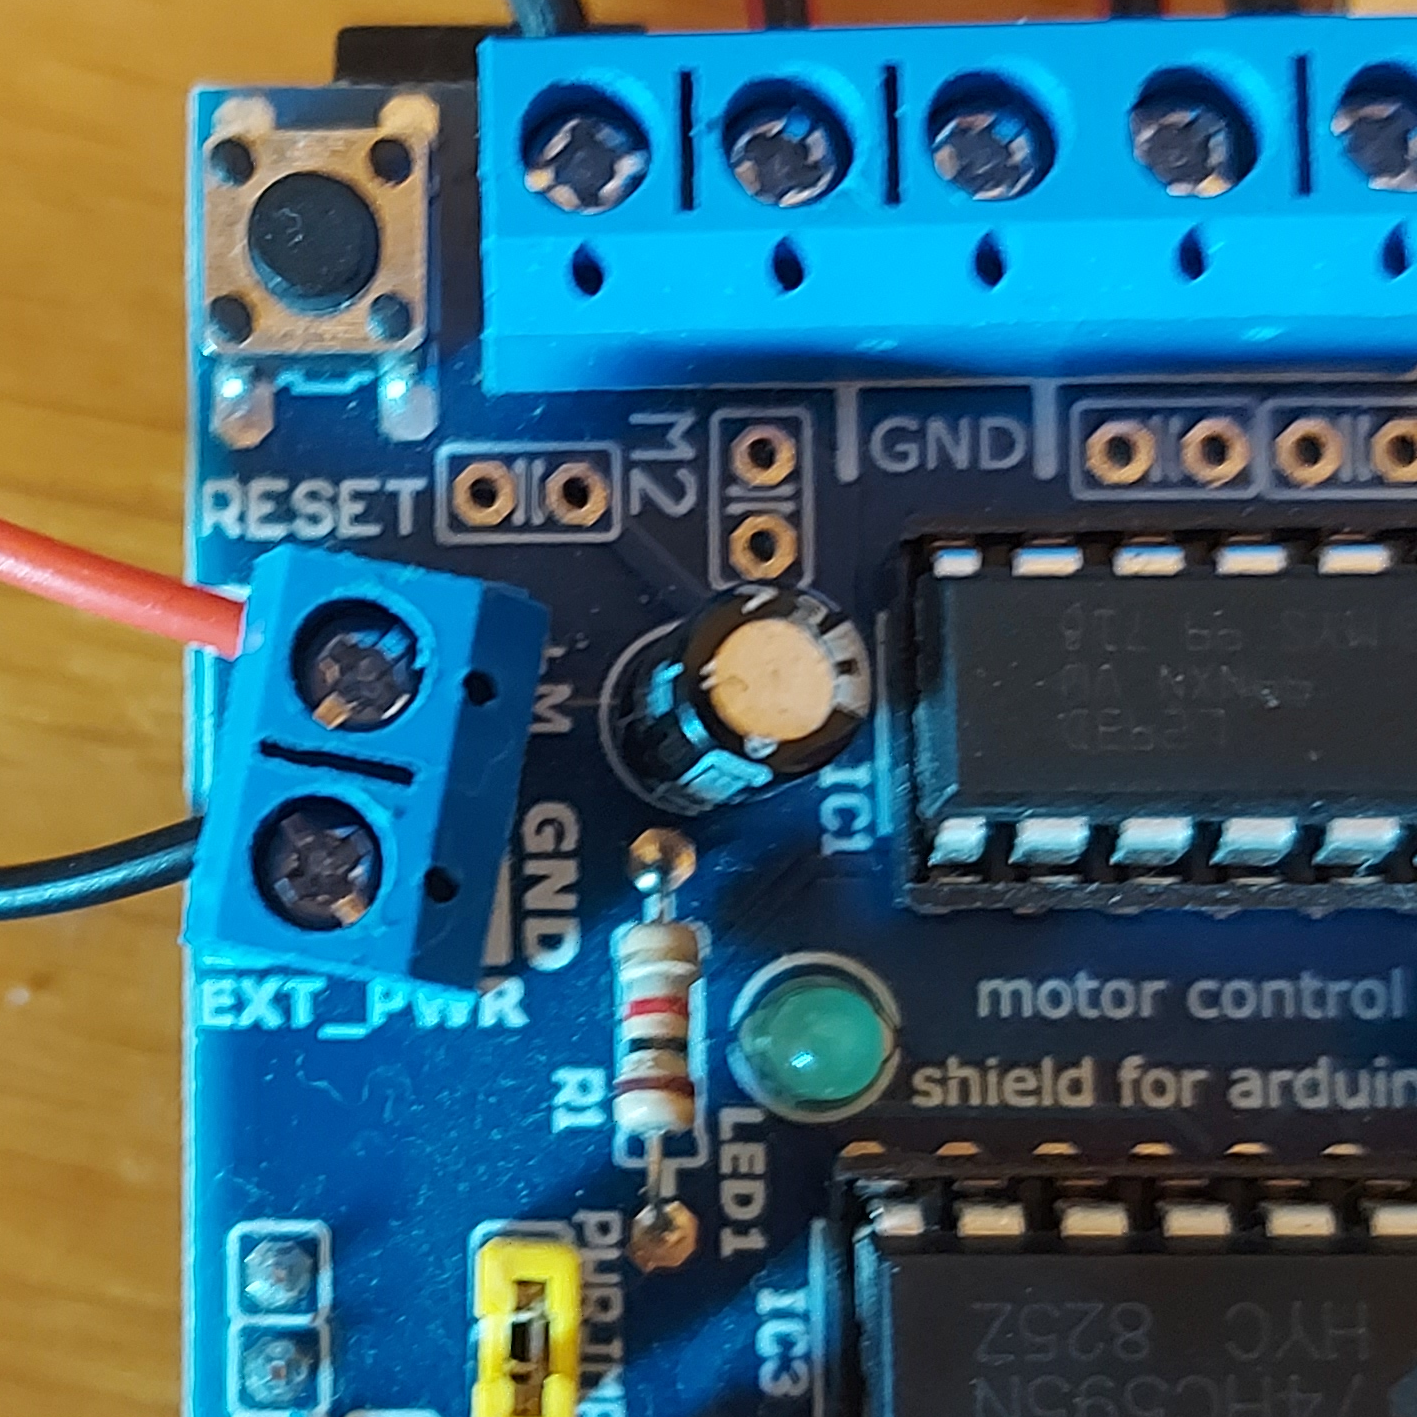
\includegraphics[width=5cm]{images/robot_build/akku-connect}
	\caption{Bekötés}
	\label{akku}
\end{figure}

\subsection{A program telepítése az alaplapra}
Csatlakoztassuk a mikrokontrollert a számtógéphez. Nyissuk meg a letöltött mappában található ’.ino’ kiterjesztésű fájlt az Arduino IDE segítségével. Az Eszközök -> Alaplap menüpontban válasszuk ki a használt alaplap típusát, valamint a portot amelyen keresztül csatlakoztattuk a számítógéphez. Kattintsunk a feltöltés gombra. 

Amint elkészül a feltöltés az IDE jelzi, ezek után az alaplapot leválaszthatjuk. Utolsó lépésként helyezzük el a mikrokontrollert a roboton, majd csatlakoztassuk hozzá a shield-et, ezek után a robot működőképes.
\section{A telefonon elvégzendő lépések}
Mielőtt a robotot vezérelni tudnánk el kell végeznünk néhány lépést.
\subsection{Az alkalmazás telepítése}
Mivel az alkalmazás még nem érhető el a PlayStore-on, ezért a telepítést manuálisan kell elvégeznünk. Ennek menete:
\begin{itemize}
	\item A számítógépről másoljuk a készülékre az 'app-debug.apk' nevű fájlt
	\item Engedélyezzük a Beállításokban az ismeretlen forrásból származó alkalmazások telepítését
	\item Nyissuk meg a telefon fájlkezelő programját, majd keressük ki és futassuk a fájlt.
	\item A megjelenő üzenetetnél válasszuk a 'Telepítés' lehetőséget
	\item Az installálás közben felugró 'PlayProtect' üzenetkor válasszuk a 'Telepítés mégis' opciót
	\item Amennyiben megkapjuk az 'Alkalmazás telepítve' üzenetet a telepítés sikeres volt, használhatjuk az alkalmazást
\end{itemize}

Fontos megjegyezni, hogy a sikertelen telepítés főbb okai a következők lehetnek:
\begin{itemize}
	\item A telefon nem rendelkezik elegendő szabad tárhellyel
	\item Az alkalmazás nem kompatibilis a készülék Android verziójával
	\item Nem engedélyezett az ismeretlen forrásból származó alkalmazások telepítése
\end{itemize}
\subsection{Bluetooth párosítás}
Ahhoz, hogy a robothoz csatlakozni tudjunk először párosítani kell a készülékünket a roboton található HC-05 modullal. Ezt úgy tudjuk megtenni, hogy a telefonon elnavigálunk a Beállítások $\rightarrow$ Kapcsolatok $\rightarrow$ Bluetooth menüpontra, majd bekapcsoljuk a telefonban található Bluetooth egységet.

Ezek után a roboton bekapcsoljuk az akkumulátort, ezzel energiával látjuk el a HC-05-ös modult, ami ezt követően megjelenik az elérhető eszközök listájában.

A párosításhoz ki kell választanunk az eszközt és a felugró párbeszédablakban jelszónak az '1234' számsort kell beírnunk. Amint a párosítás megtörtént az applikációt indíthatjuk.
\subsection{Az alkalmazás első indítása}
Az alkalmazás indítását követően a kezdőképernyő fogad minket (lásd \ref{home-screen}~ábra).Itt az ,,Eszközök'' gomb megnyomása után láthatóvá válik a párosított eszközök listája.

Miután kiválasztottuk a HC-05-ös szenzort a listából a ,,Követés'', ,,Irányítás'' és ,,Log'' gombok valamelyikét megnyomva a telefon csatlakozik a robothoz.

Amennyiben a ,,Log'' gombot választjuk az applikáció a Naplózási képernyőre navigál minket, ahol az első futtatás alkalmával engedélyt kell adnunk az applikációnak a tárhely eléréséhez. Ha ezt nem tesszük meg a Naplófájlt nem fogjuk tudni menteni mindaddig, amíg az engedélyt meg nem adjuk.
\begin{figure}[h]
	\centering
	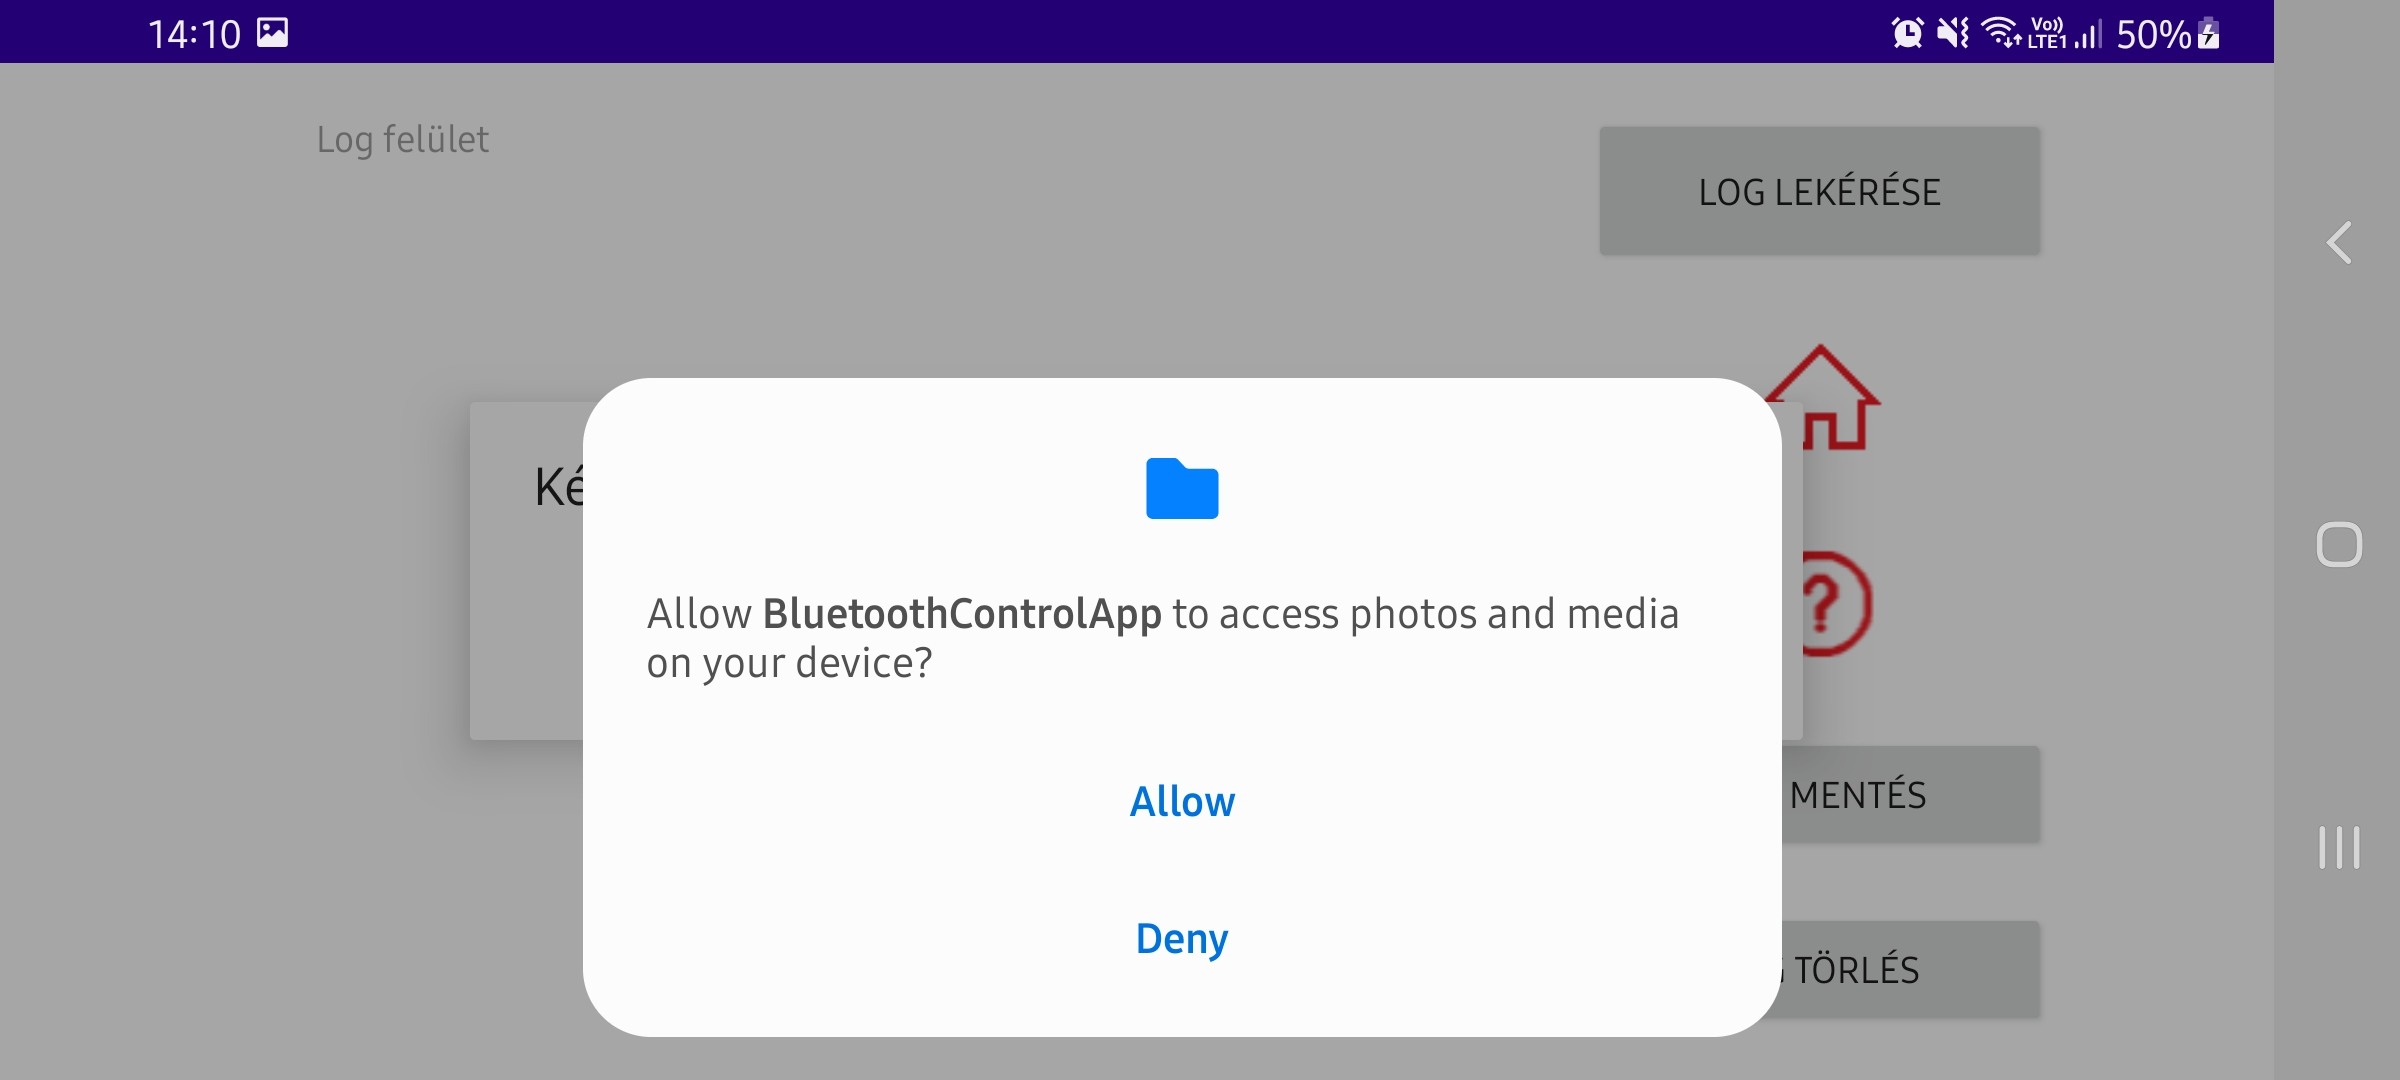
\includegraphics[width=\columnwidth]{images/app_screen/permission_grant}
	\caption{Engedélyadás}
	\label{grant_permission}
\end{figure}

Ezek után az applikáció minden funkciója használható.
\begin{thebibliography}{1}
	\bibitem{Wikipedia_Arduino}  \textsc{\url{https://hu.wikipedia.org/wiki/Arduino}}
	\bibitem{Arduino IDE} \textsc{\url{https://www.arduino.cc/en/Guide/Environment}}
	\bibitem{Wikipedia_CPP}
	\textsc{\url{https://hu.wikipedia.org/wiki/C\%2B\%2B}}
	\bibitem{Wikipedia_Android}
	\textsc{\url{https://hu.wikipedia.org/wiki/Android\_(operációs\_rendszer)}}
	\bibitem{Wikipedia_Android_Studio}
	\textsc{\url{https://hu.wikipedia.org/wiki/Android\_Studio}}
	\bibitem{Wikipedia_Java}
	\textsc{\url{https://hu.wikipedia.org/wiki/Java\_(programozási\_nyelv)}}
	\bibitem{Ultrahang_Szenzor}
	\textsc{\url{https://create.arduino.cc/projecthub/abdularbi17/ultrasonic-sensor-hc-sr04-with-arduino-tutorial-327ff6}}
	\bibitem{Bluetooth_active}
	\textsc{\url{https://stackoverflow.com/questions/7672334/how-to-check-if-bluetooth-is-enabled-programmatically}}
	\bibitem{Bluetooth_enable}
	\textsc{\url{https://stackoverflow.com/questions/3806536/how-to-enable-disable-bluetooth-programmatically-in-android}}
	\bibitem{Bluetooth_connect}
	\textsc{\url{https://stackoverflow.com/questions/5171248/programmatically-connect-to-paired-bluetooth-device}}
\end{thebibliography}
\end{document}